%%%%%%%%%%
% if Appendix is needed:
%%%%%%%%%%
\renewcommand{\theHchapter}{A\arabic{chapter}}
\appendix
%	\begin{appendices}
\phantomsection

\chapter{Model Measurements}
\label{app:model_measurements}
  \begin{table}
    \centering
    \begin{tabular}{lrl}
    Name & Dimension & Unit [in] \\
    fuselage & Length & $18$\\
            & Diameter &  $3$\\
            & Fin     & $2 \frac{5}{16}$\\
            \\
    Nose-1  & Base & $3$ \\
            & Edge Length & $3 \frac{11}{16}$ \\
            \\
    Nose-2  & Base & $3$ \\
            & Edge Length & $5 \frac{13}{16}$ \\
            \\
    Nose-3  & Base & $3$ \\
            & Edge Length & $8 \frac{11}{16}$ \\
            \\
    Nose-4  & Base & $3$ \\
            & Diameter 1 & $2.91339$ \\
            & Diameter 2 & $2.56$ \\
            & Diameter 3 & $1.57$ \\
            \\
    Nose-5  & Base & $3$ \\
            & Diameter 1 & $2.87$ \\
            & Diameter 2 & $2.52$ \\
            & Diameter 3 & $1.89$ \\
            & Diameter 3 & $0.83$ \\
    \end{tabular}
    \caption{Model dimensions}
    \label{tab:models}
  \end{table}

\chapter{Models}
\label{app:models}

  \begin{figure}[htbp]
    \centering
    \begin{subfigure}{.5\textwidth}
      \centering
      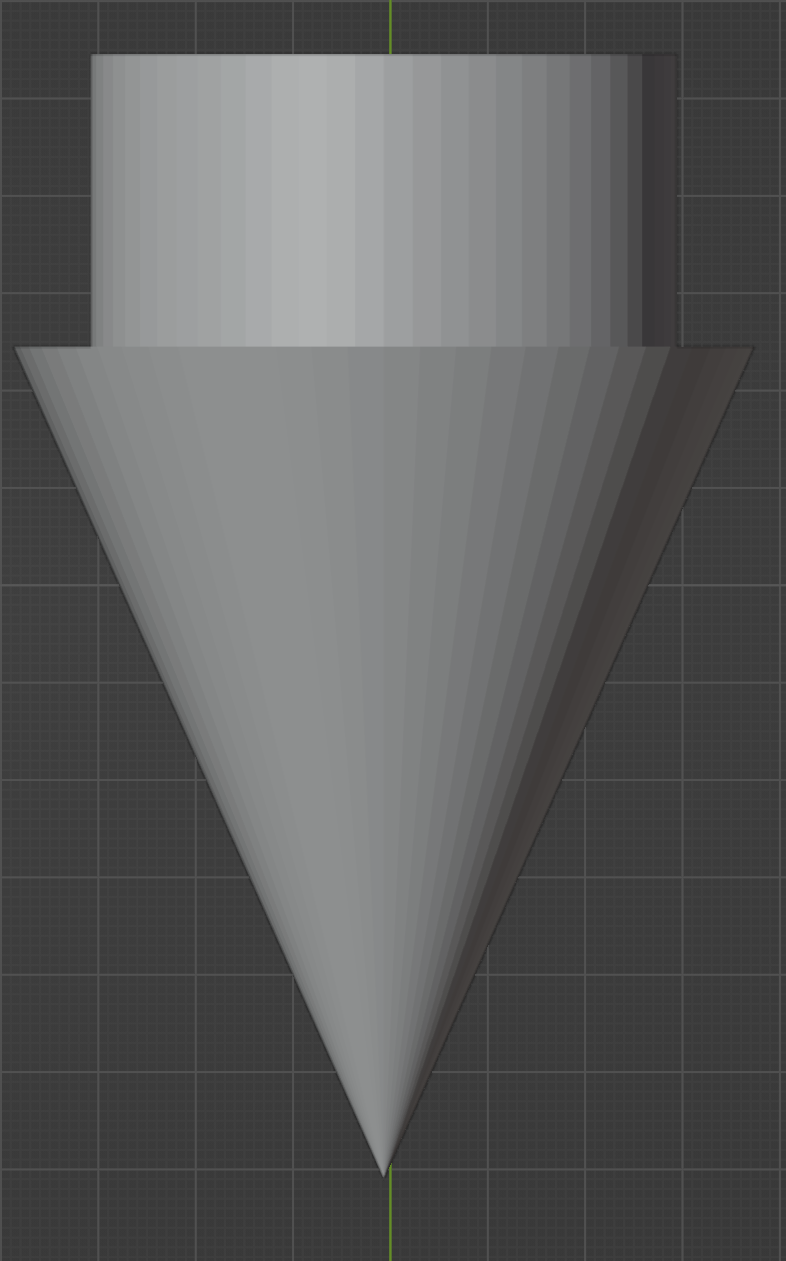
\includegraphics[width=.8\linewidth]{nose_1.png}
    \end{subfigure}%
    \begin{subfigure}{.5\textwidth}
      \centering
      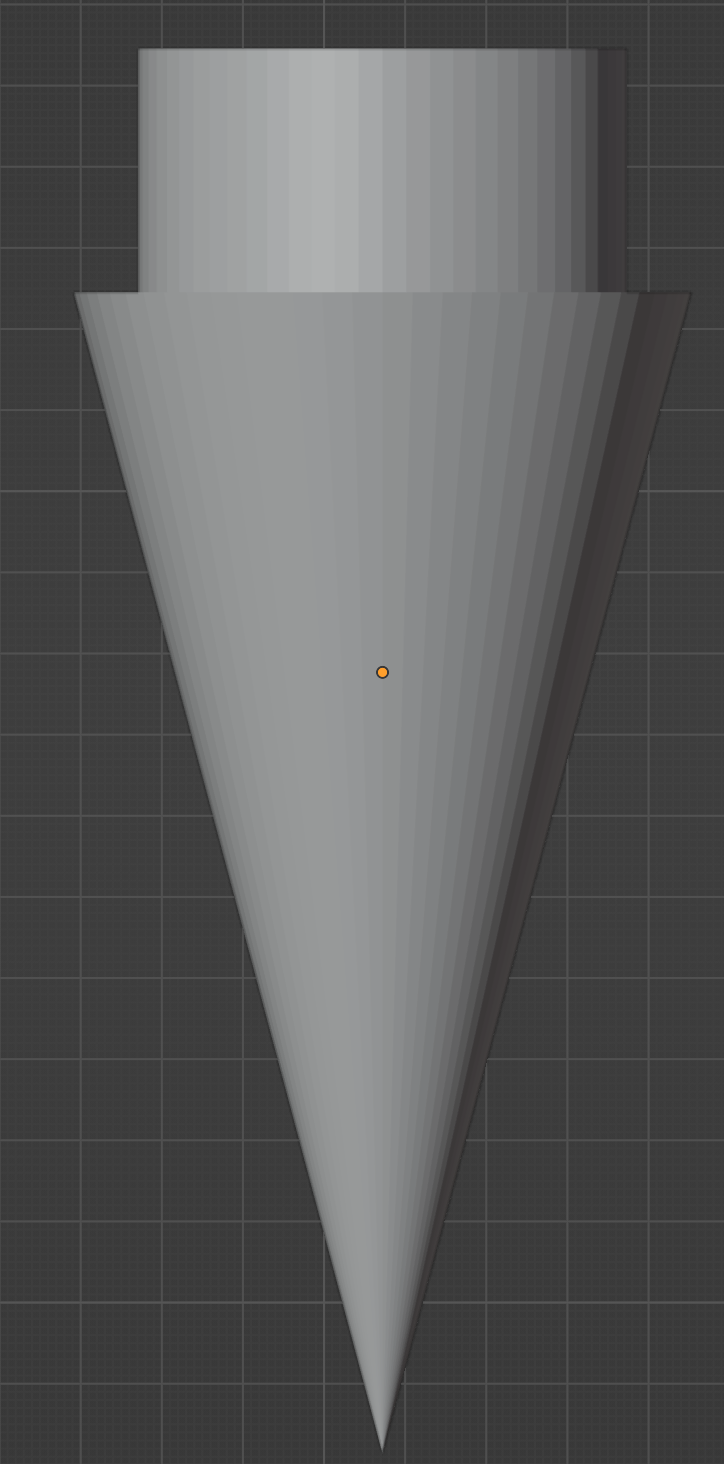
\includegraphics[width=.8\linewidth]{nose_2.png}
    \end{subfigure}
    \caption{Simulation targets 1 and 2}
    \label{fig:nose_1_2}
  \end{figure}

  \begin{figure}[htbp]
    \centering
    \begin{subfigure}{.5\textwidth}
      \centering
      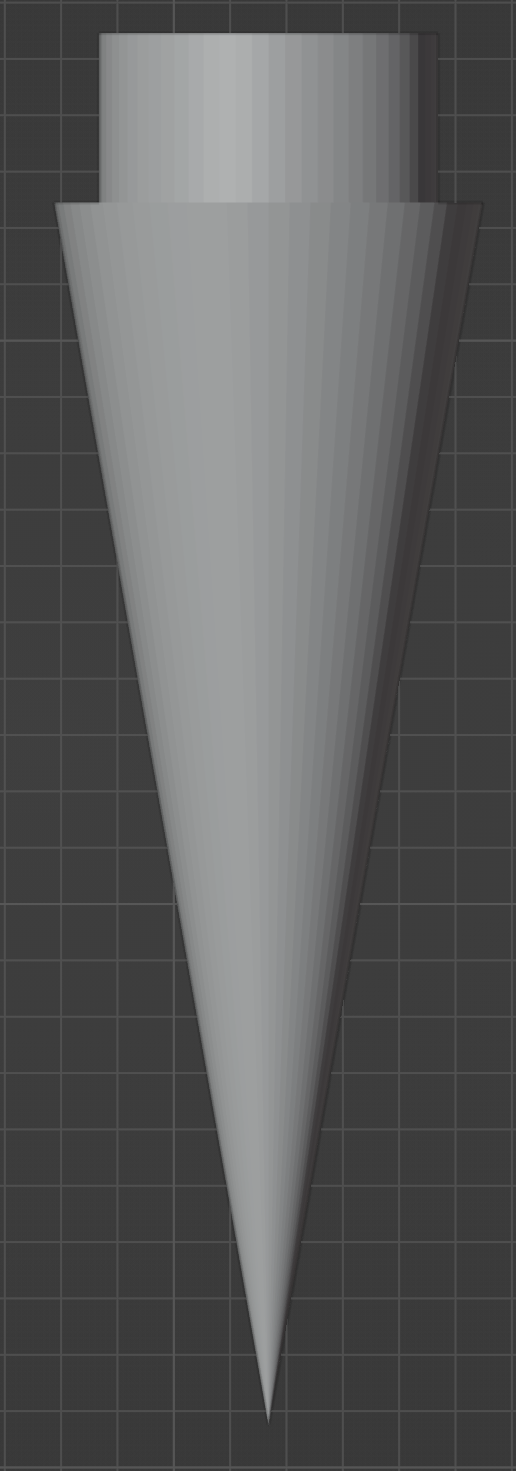
\includegraphics[width=.8\linewidth]{nose_3.png}
    \end{subfigure}%
    \begin{subfigure}{.5\textwidth}
      \centering
      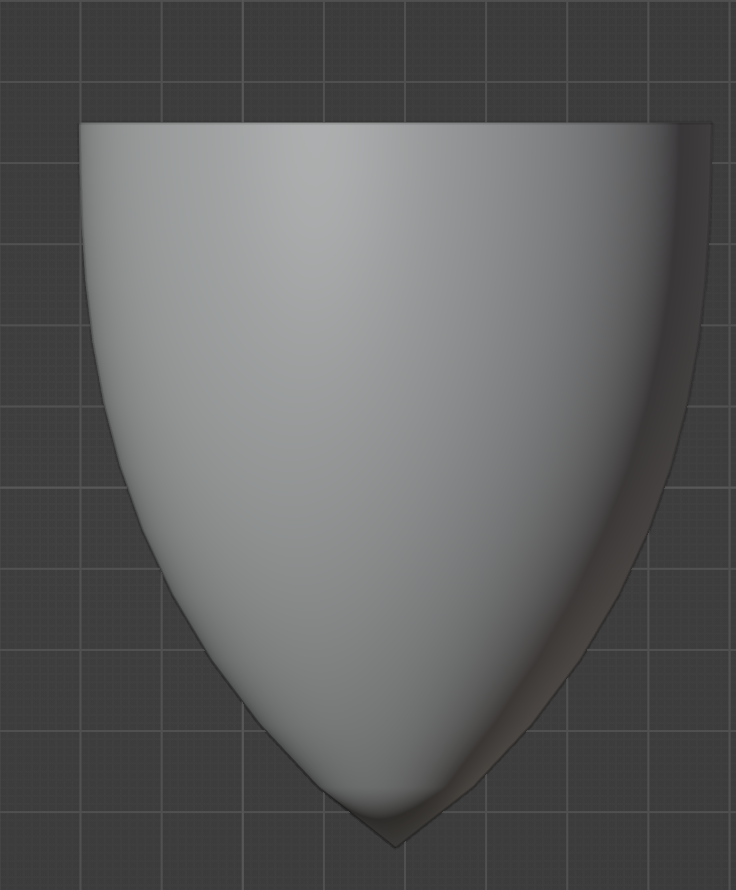
\includegraphics[width=.8\linewidth]{nose_4.png}
    \end{subfigure}
    \caption{Simulation targets 3 and 4}
    \label{fig:nose_3_4}
  \end{figure}

  \begin{figure}[htbp]
    \centering
    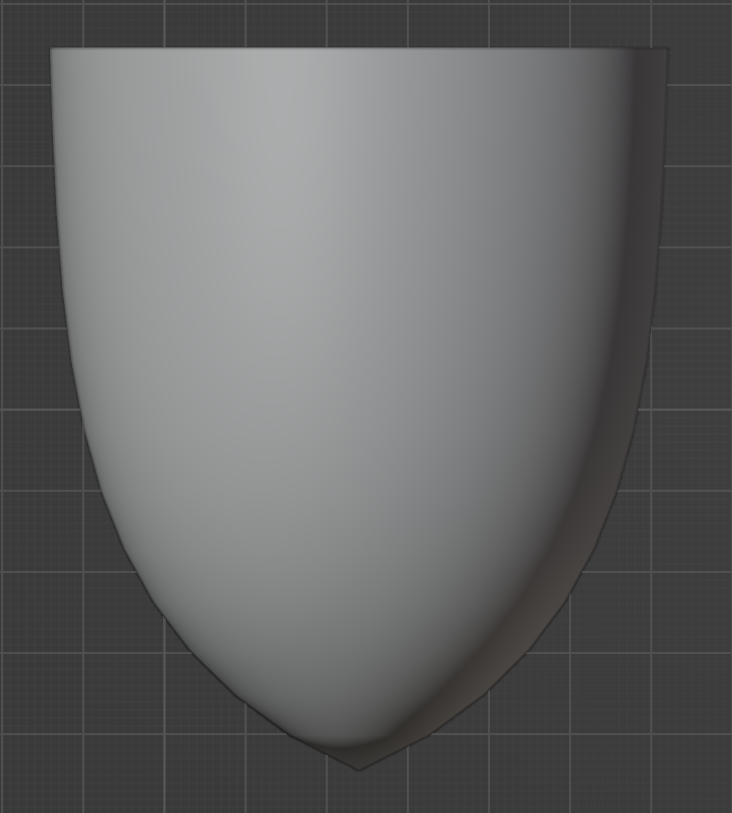
\includegraphics[width=.8\linewidth]{nose_5.png}
    \caption{Simulation targets 3 and 4}
    \label{fig:nose_5}
  \end{figure}

\chapter{Measurement Results}
\label{app:measurement_results}
  \begin{figure}[htbp]
    \centering
    \begin{subfigure}{.5\textwidth}
      \centering
      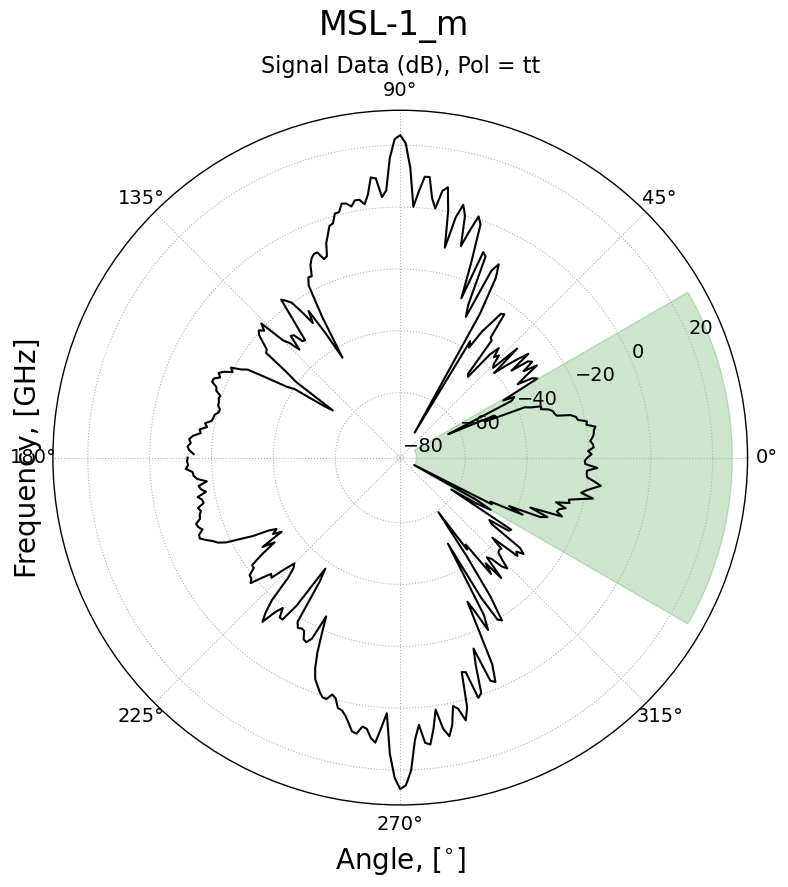
\includegraphics[width=.8\linewidth]{MSL-1_m_dB_tt_5GHz.png}
    \end{subfigure}%
    \begin{subfigure}{.5\textwidth}
      \centering
      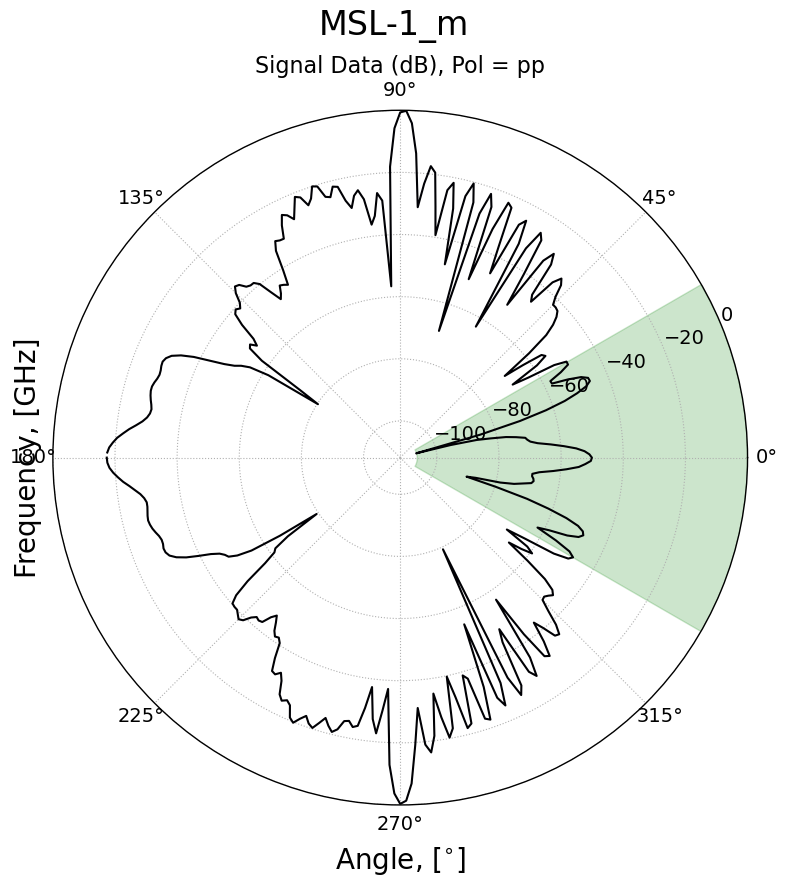
\includegraphics[width=.8\linewidth]{MSL-1_m_dB_pp_5GHz.png}
    \end{subfigure}
    \caption{Missile 1 \textcolor{green}{(Test)}:  RCS cut at 5 GHz. Vertical (tt) and Horizontal (pp) polarizations }
    \label{fig:n1}
  \end{figure}

  \begin{figure}[htbp]
    \centering
    \begin{subfigure}{.5\textwidth}
      \centering
      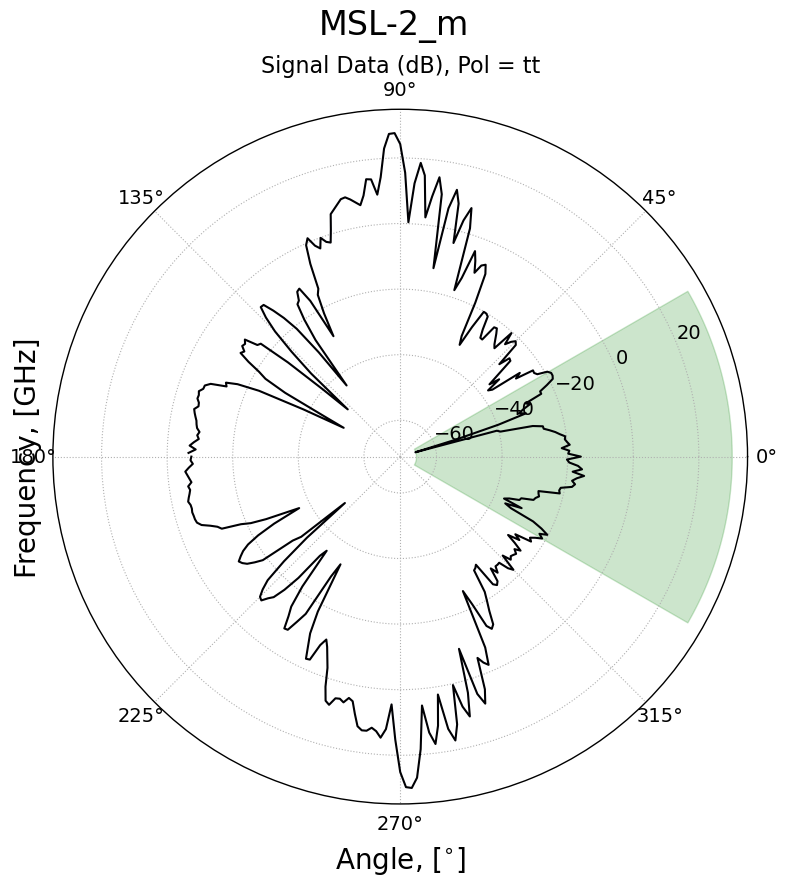
\includegraphics[width=.8\linewidth]{MSL-2_m_dB_tt_5GHz.png}
    \end{subfigure}%
    \begin{subfigure}{.5\textwidth}
      \centering
      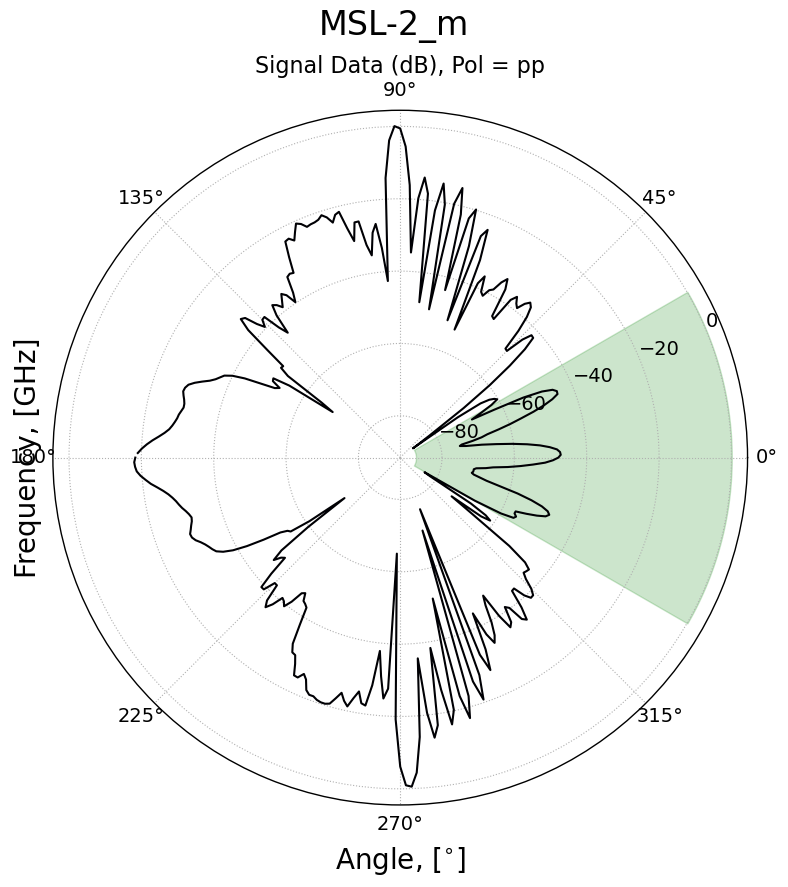
\includegraphics[width=.8\linewidth]{MSL-2_m_dB_pp_5GHz.png}
    \end{subfigure}
    \caption{Missile 2 \textcolor{green}{(Test)}:  RCS cut at 5 GHz. Vertical (tt) and Horizontal (pp) polarizations }
    \label{fig:n2}
  \end{figure}

  \begin{figure}[htbp]
    \centering
    \begin{subfigure}{.5\textwidth}
      \centering
      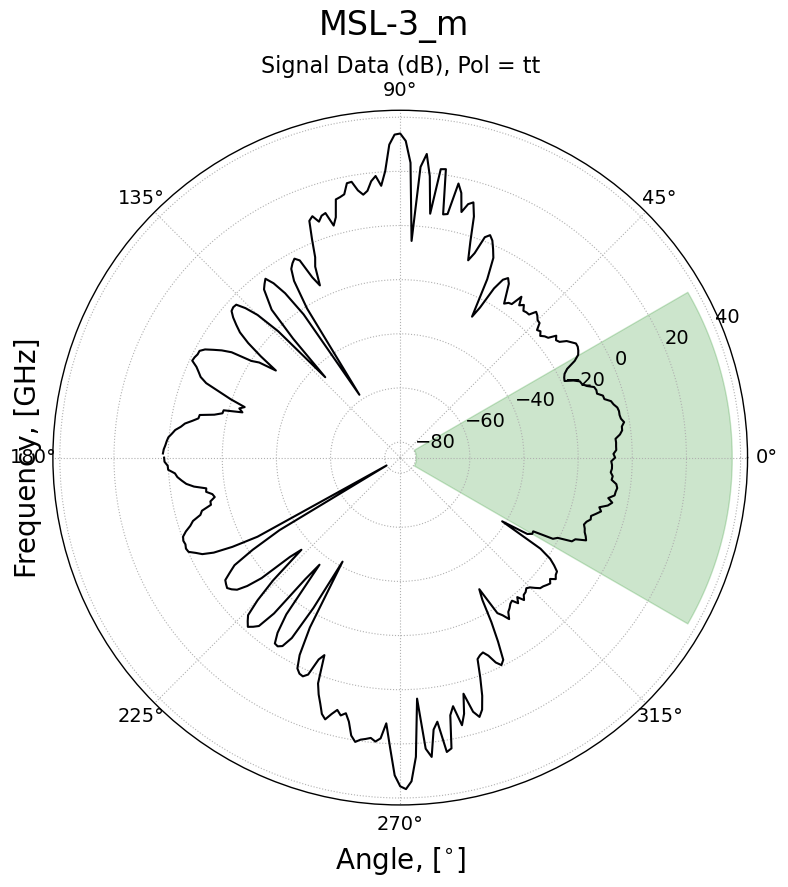
\includegraphics[width=.8\linewidth]{MSL-3_m_dB_tt_5GHz.png}
    \end{subfigure}%
    \begin{subfigure}{.5\textwidth}
      \centering
      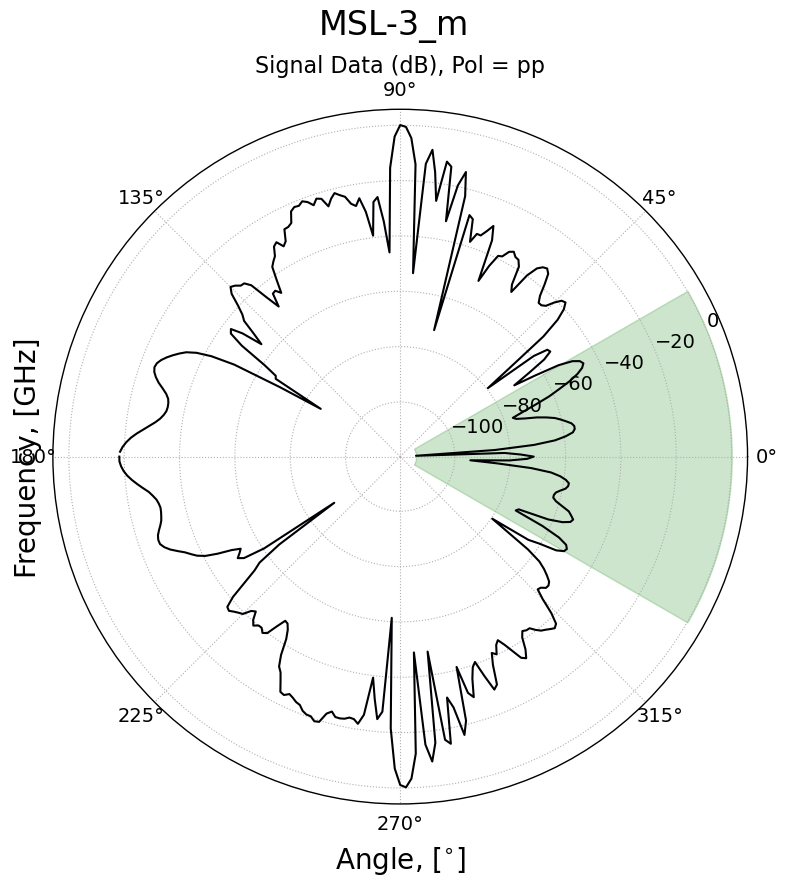
\includegraphics[width=.8\linewidth]{MSL-3_m_dB_pp_5GHz.png}
    \end{subfigure}
    \caption{Missile 3 \textcolor{green}{(Test)}:  RCS cut at 5 GHz. Vertical (tt) and Horizontal (pp) polarizations }
    \label{fig:n3}
  \end{figure}

  \begin{figure}[htbp]
    \centering
    \begin{subfigure}{.5\textwidth}
      \centering
      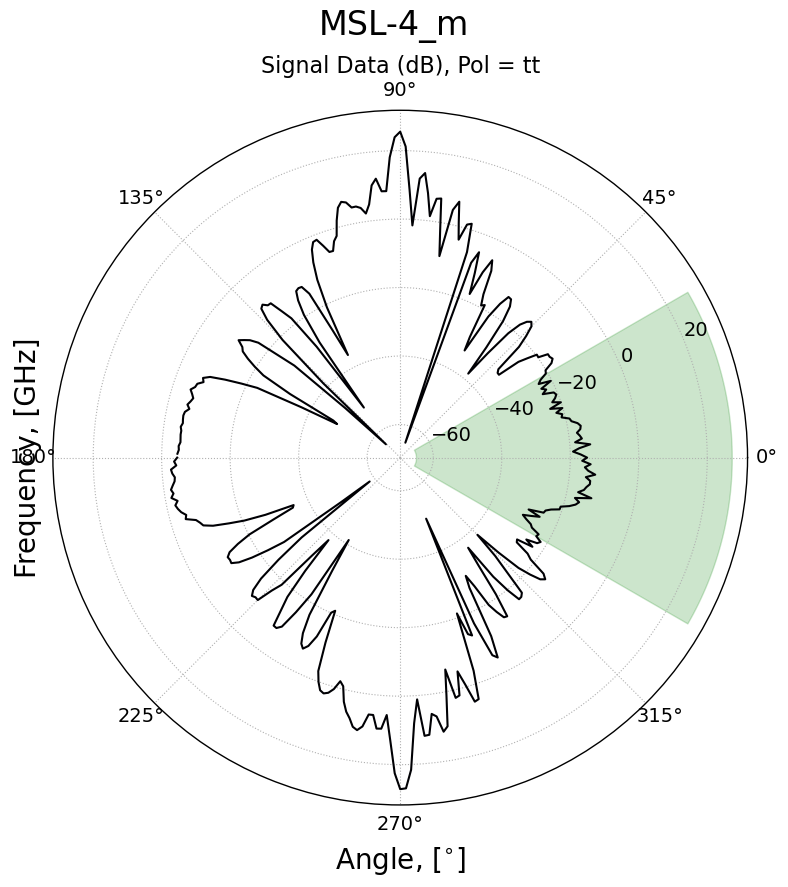
\includegraphics[width=.8\linewidth]{MSL-4_m_dB_tt_5GHz.png}
    \end{subfigure}%
    \begin{subfigure}{.5\textwidth}
      \centering
      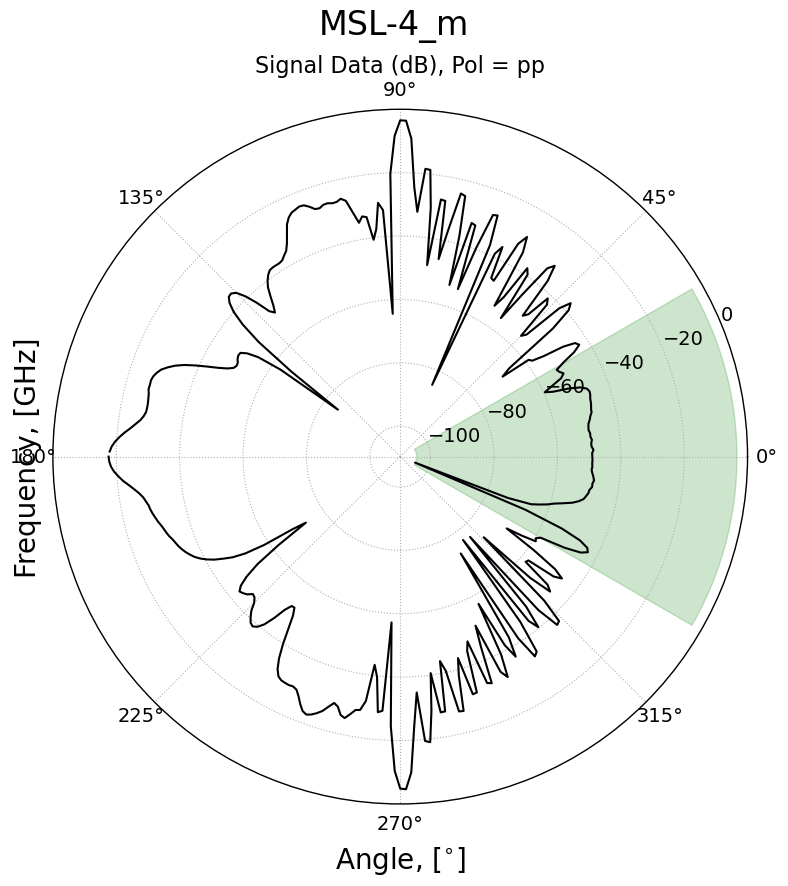
\includegraphics[width=.8\linewidth]{MSL-4_m_dB_pp_5GHz.png}
    \end{subfigure}
    \caption{Missile 4 \textcolor{green}{(Test)}:  RCS cut at 5 GHz. Vertical (tt) and Horizontal (pp) polarizations }
    \label{fig:n4}
  \end{figure}

  \begin{figure}[htbp]
    \centering
    \begin{subfigure}{.5\textwidth}
      \centering
      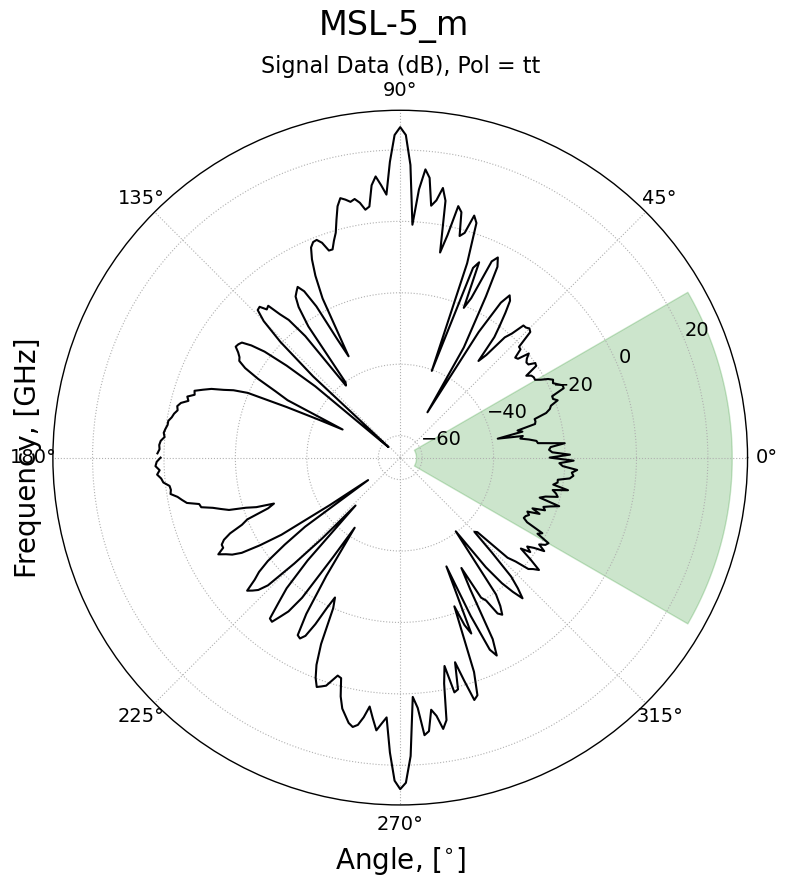
\includegraphics[width=.8\linewidth]{MSL-5_m_dB_tt_5GHz.png}
    \end{subfigure}%
    \begin{subfigure}{.5\textwidth}
      \centering
      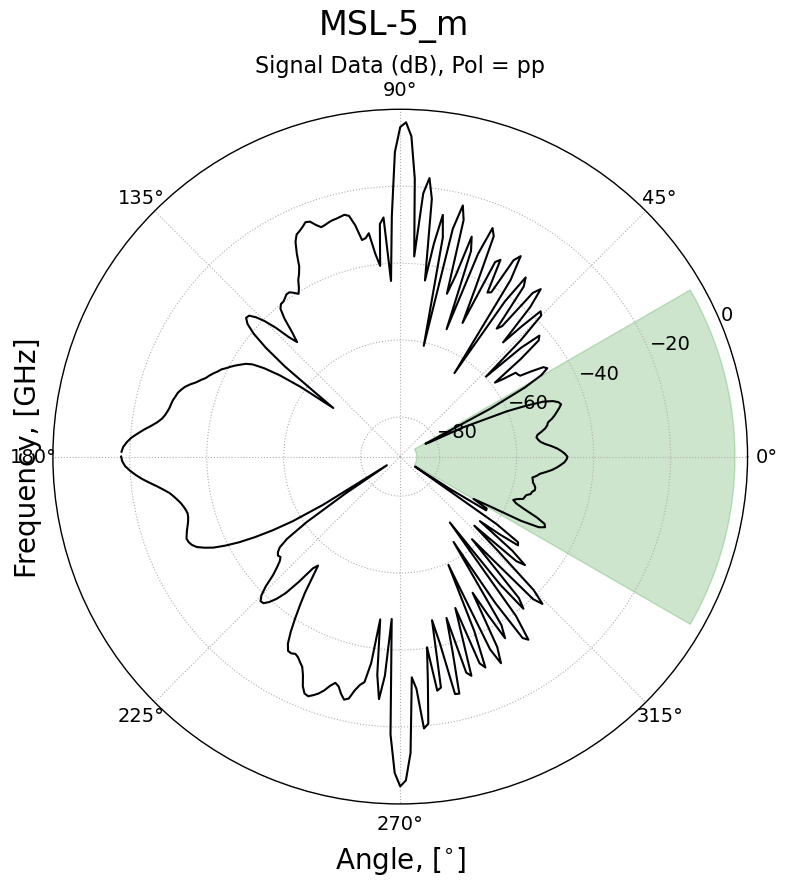
\includegraphics[width=.8\linewidth]{MSL-5_m_dB_pp_5GHz.png}
    \end{subfigure}
    \caption{Missile 5 \textcolor{green}{(Test)}:  RCS cut at 5 GHz. Vertical (tt) and Horizontal (pp) polarizations }
    \label{fig:n5}
  \end{figure}

  \begin{figure}[htbp]
    \centering
    \begin{subfigure}{.5\textwidth}
      \centering
      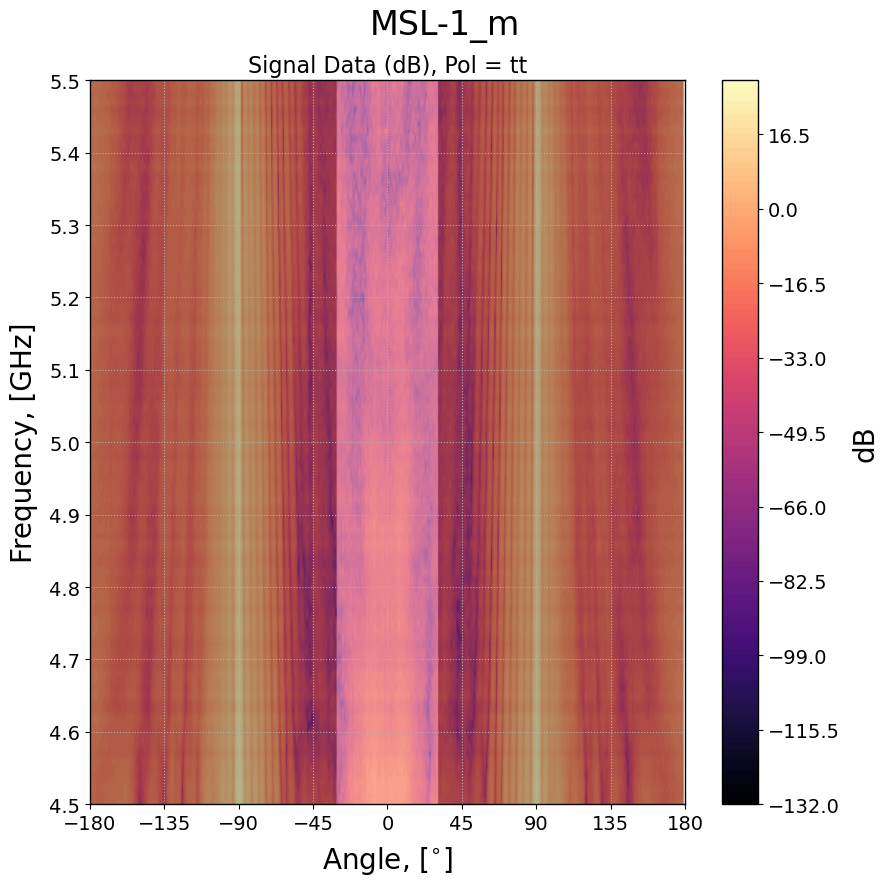
\includegraphics[width=.8\linewidth]{MSL-1_m_dB_tt.png}
    \end{subfigure}%
    \begin{subfigure}{.5\textwidth}
      \centering
      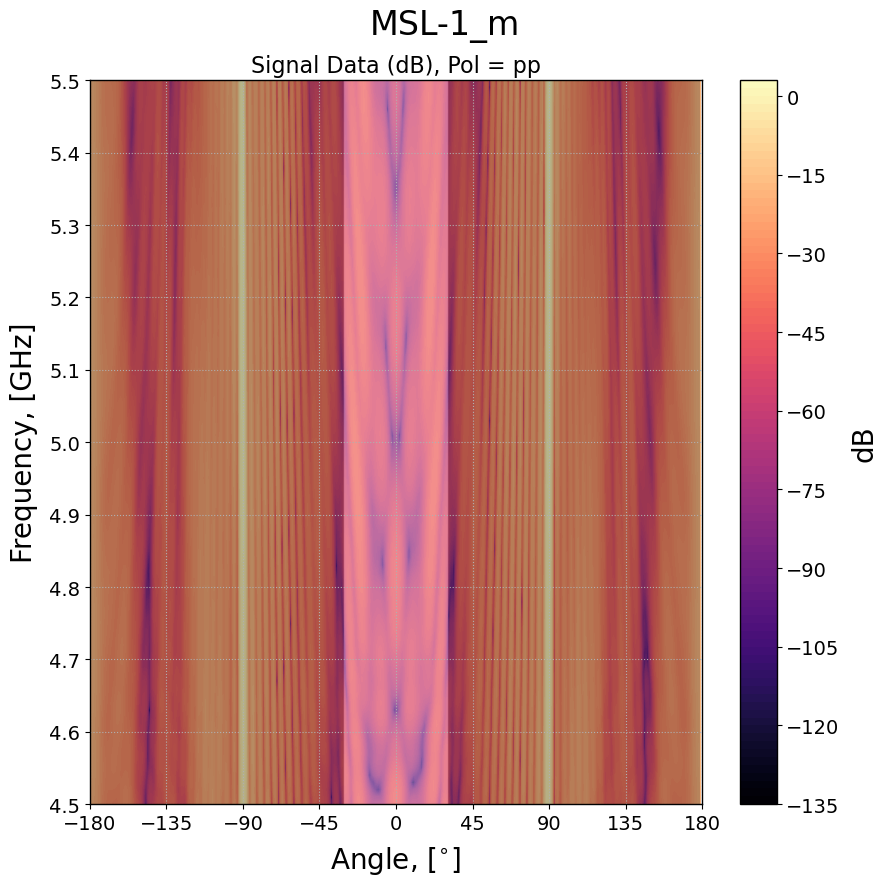
\includegraphics[width=.8\linewidth]{MSL-1_m_dB_pp.png}
    \end{subfigure}
    \caption{Missile 1 \textcolor{green}{(Test)}:  Total RCS. Vertical (tt) and Horizontal (pp) polarizations }
    \label{fig:c1}
  \end{figure}

  \begin{figure}[htbp]
    \centering
    \begin{subfigure}{.5\textwidth}
      \centering
      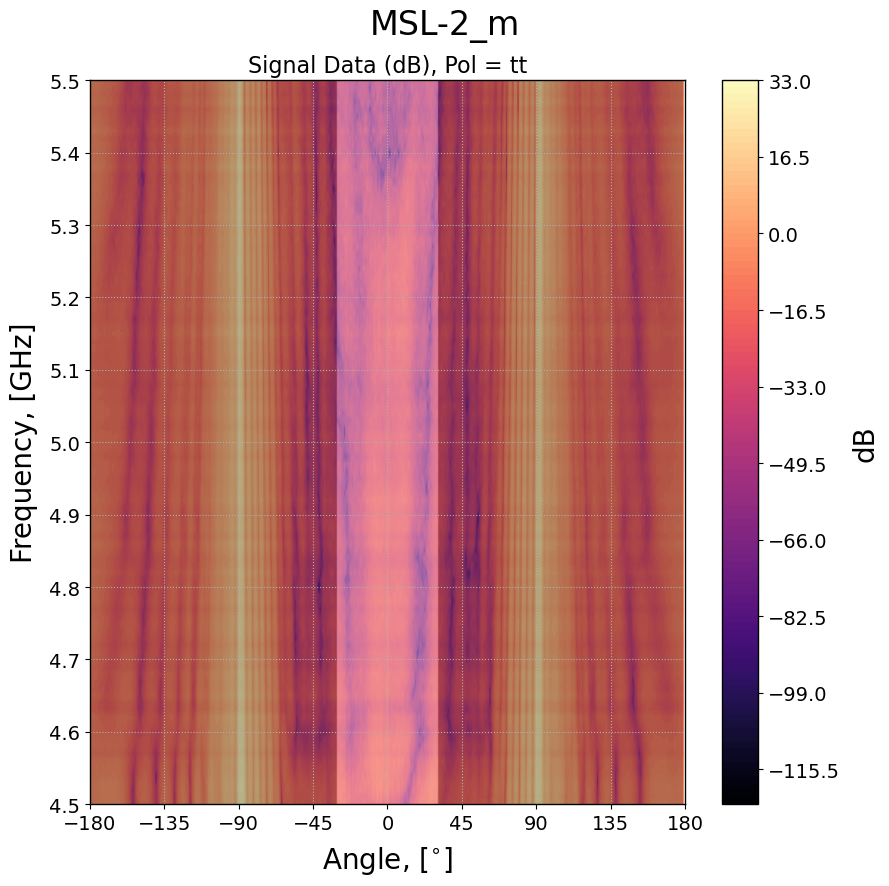
\includegraphics[width=.8\linewidth]{MSL-2_m_dB_tt.png}
    \end{subfigure}%
    \begin{subfigure}{.5\textwidth}
      \centering
      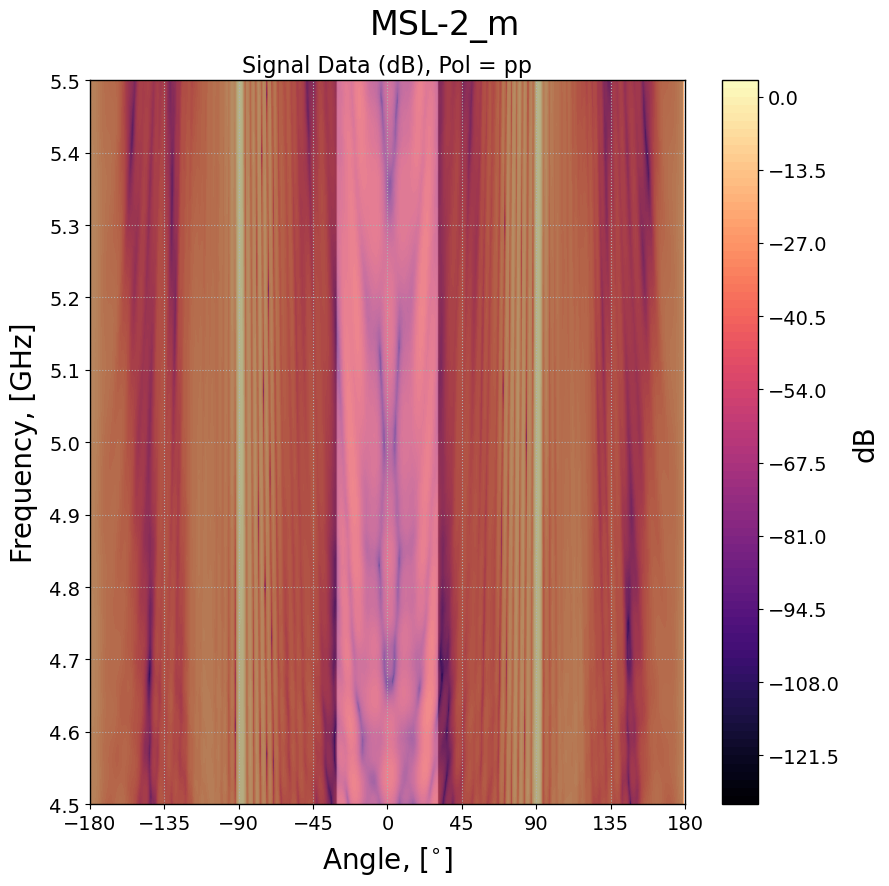
\includegraphics[width=.8\linewidth]{MSL-2_m_dB_pp.png}
    \end{subfigure}
    \caption{Missile 2 \textcolor{green}{(Test)}:  Total RCS. Vertical (tt) and Horizontal (pp) polarizations }
    \label{fig:c2}
  \end{figure}

  \begin{figure}[htbp]
    \centering
    \begin{subfigure}{.5\textwidth}
      \centering
      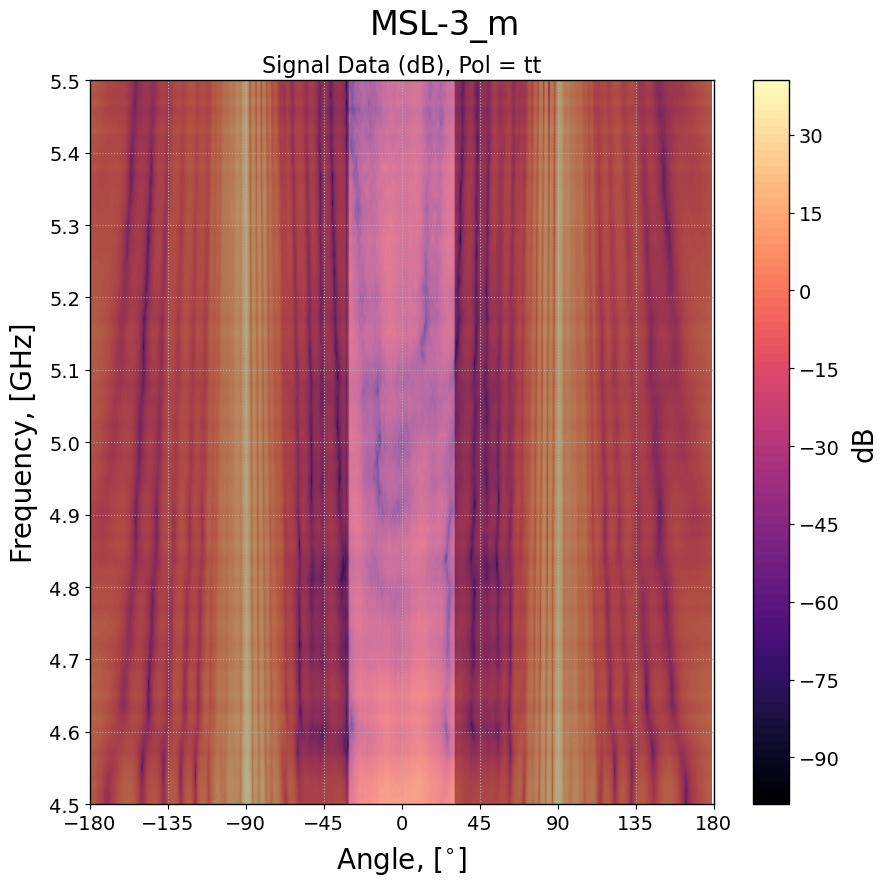
\includegraphics[width=.8\linewidth]{MSL-3_m_dB_tt.png}
    \end{subfigure}%
    \begin{subfigure}{.5\textwidth}
      \centering
      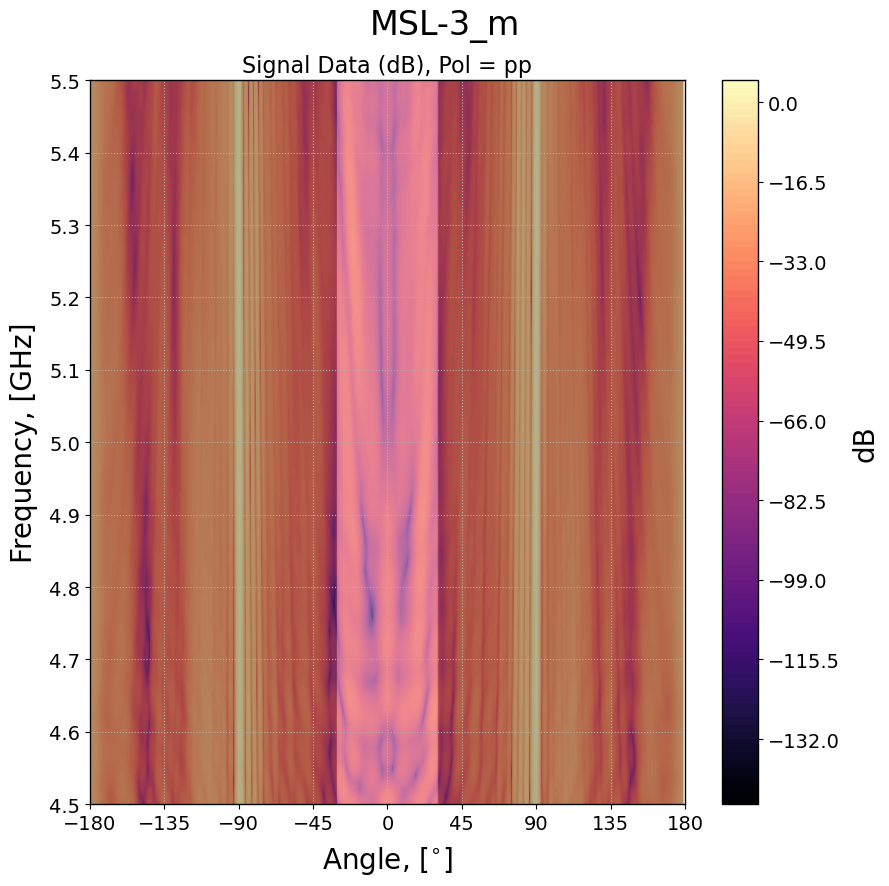
\includegraphics[width=.8\linewidth]{MSL-3_m_dB_pp.png}
    \end{subfigure}
    \caption{Missile 3 \textcolor{green}{(Test)}:  Total RCS. Vertical (tt) and Horizontal (pp) polarizations }
    \label{fig:c3}
  \end{figure}

  \begin{figure}[htbp]
    \centering
    \begin{subfigure}{.5\textwidth}
      \centering
      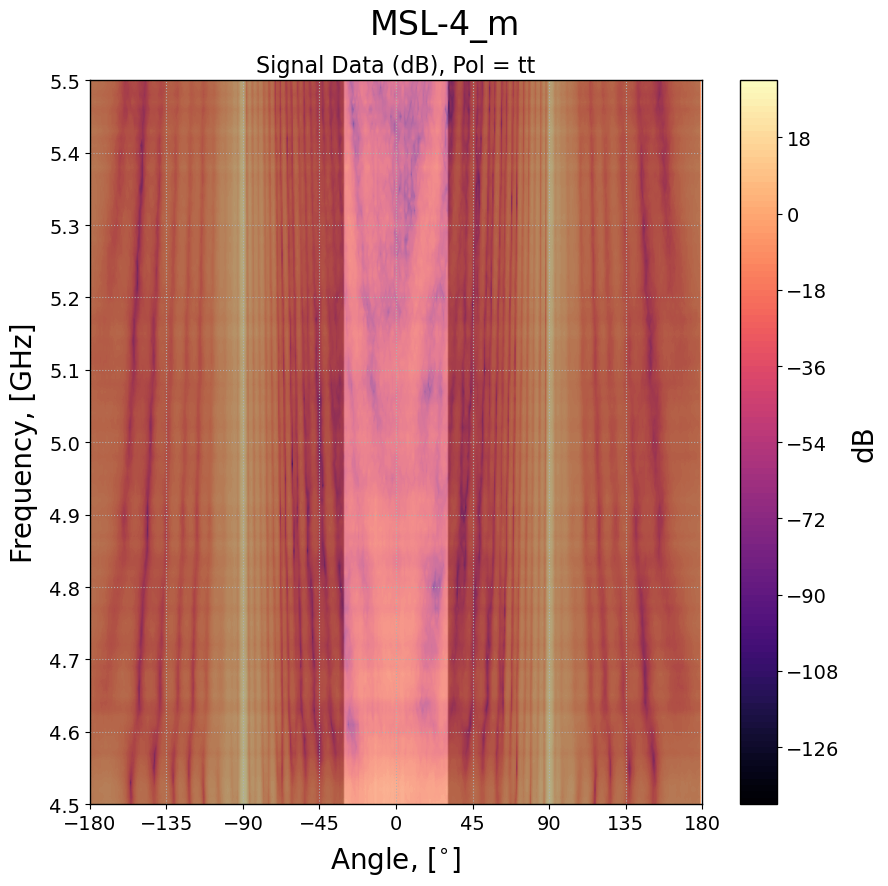
\includegraphics[width=.8\linewidth]{MSL-4_m_dB_tt.png}
    \end{subfigure}%
    \begin{subfigure}{.5\textwidth}
      \centering
      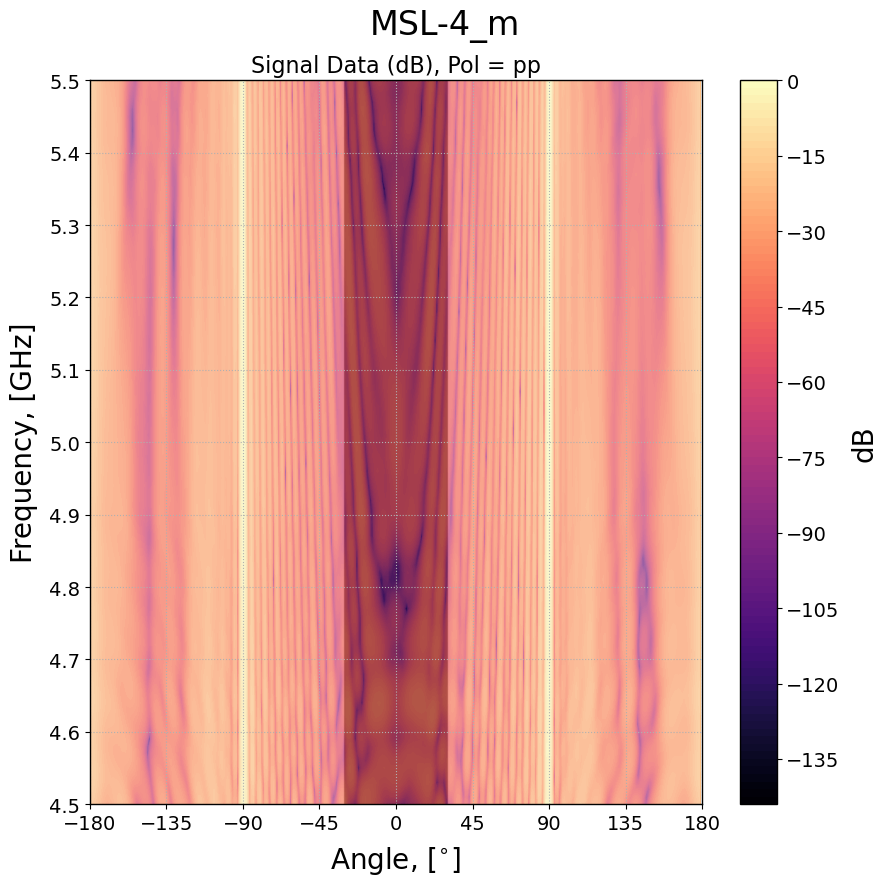
\includegraphics[width=.8\linewidth]{MSL-4_m_dB_pp.png}
    \end{subfigure}
    \caption{Missile 4 \textcolor{green}{(Test)}:  Total RCS. Vertical (tt) and Horizontal (pp) polarizations }
    \label{fig:c4}
  \end{figure}

  \begin{figure}[htbp]
    \centering
    \begin{subfigure}{.5\textwidth}
      \centering
      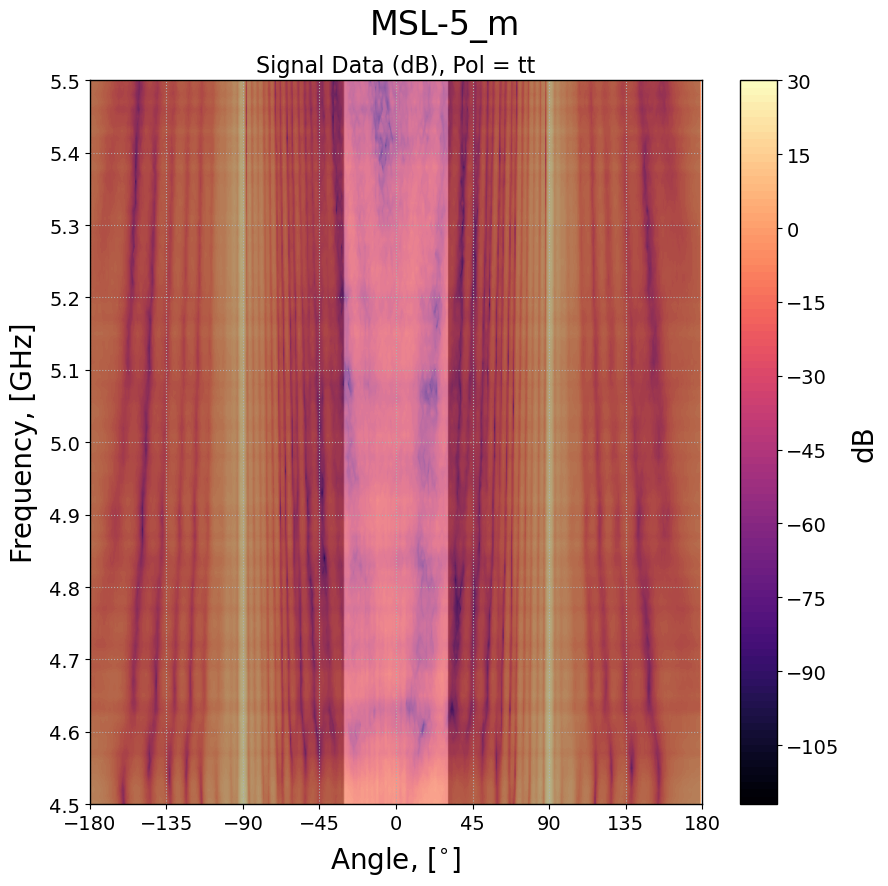
\includegraphics[width=.8\linewidth]{MSL-5_m_dB_tt.png}
    \end{subfigure}%
    \begin{subfigure}{.5\textwidth}
      \centering
      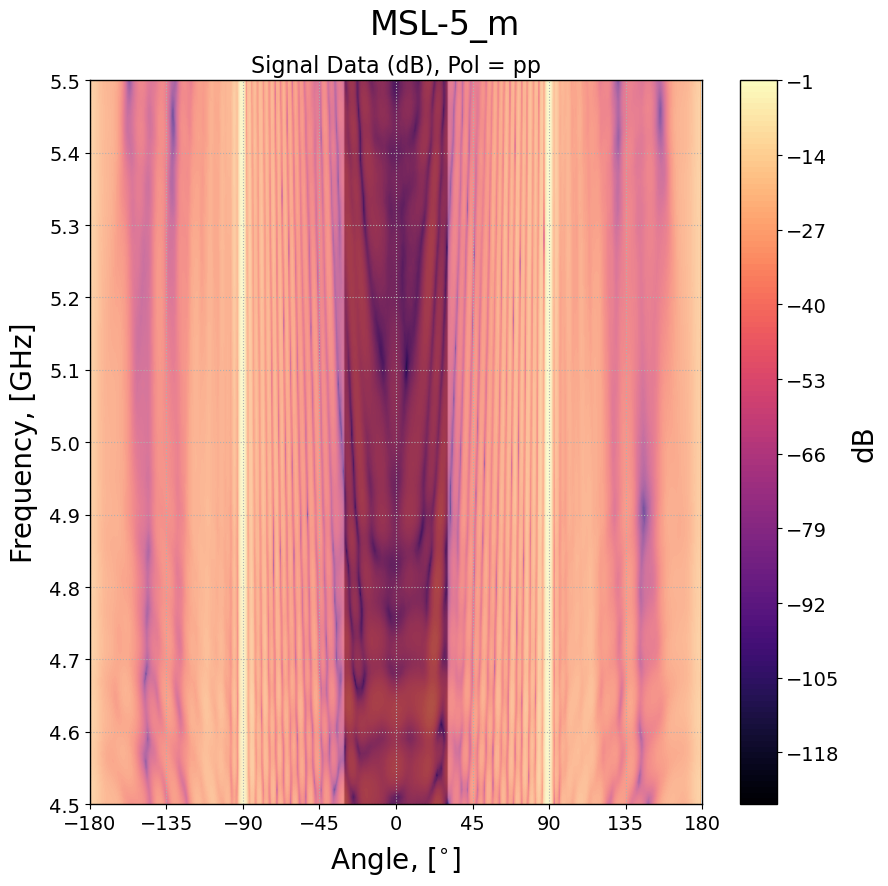
\includegraphics[width=.8\linewidth]{MSL-5_m_dB_pp.png}
    \end{subfigure}
    \caption{Missile 5 \textcolor{green}{(Test)}:  Total RCS. Vertical (tt) and Horizontal (pp) polarizations }
    \label{fig:c5}
  \end{figure}

\chapter{Simulation Results}
\label{app:simulation_results}
  \begin{figure}[htbp]
    \centering
    \begin{subfigure}{.5\textwidth}
      \centering
      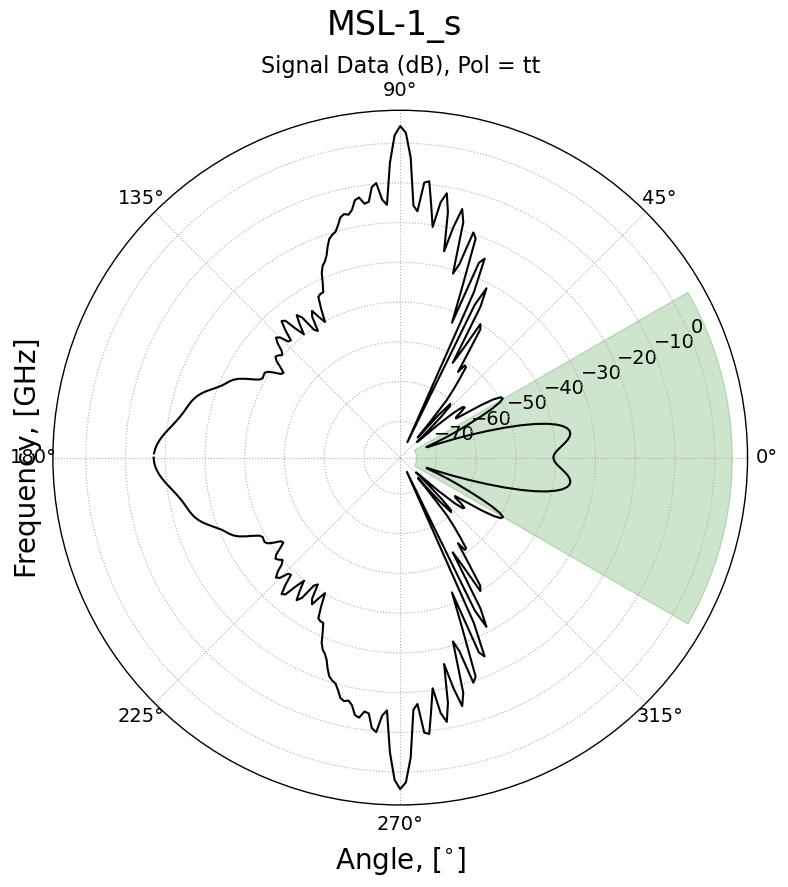
\includegraphics[width=.8\linewidth]{MSL-1_s_dB_tt_5GHz.png}
    \end{subfigure}%
    \begin{subfigure}{.5\textwidth}
      \centering
      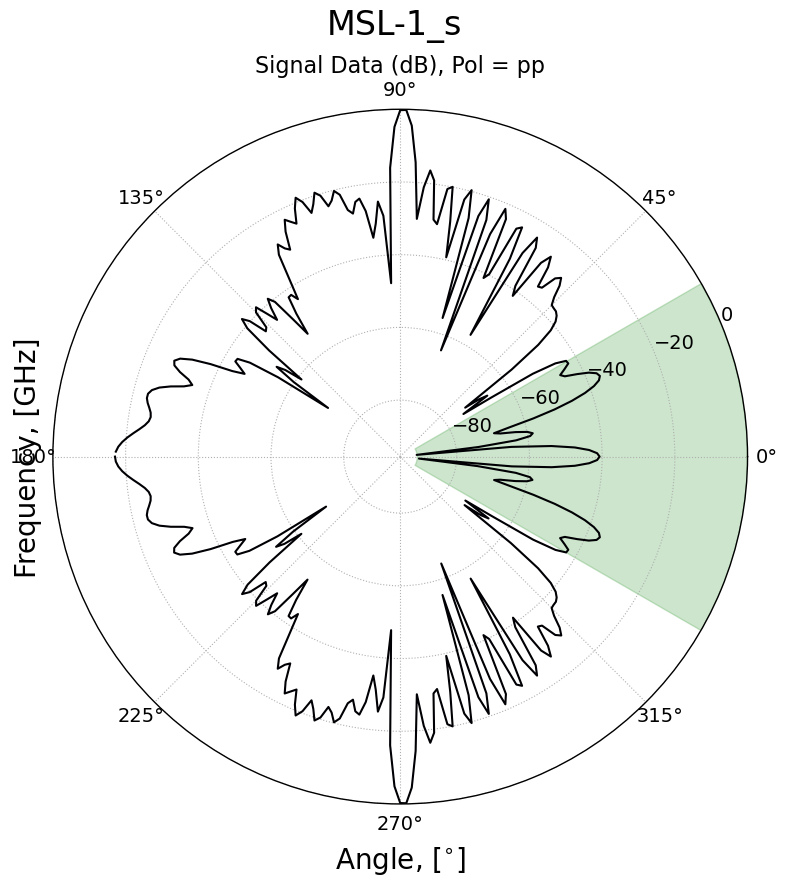
\includegraphics[width=.8\linewidth]{MSL-1_s_dB_pp_5GHz.png}
    \end{subfigure}
    \caption{Missile 1 \textcolor{red}{(Sim)}:  RCS cut at 5 GHz. Vertical (tt) and Horizontal (pp) polarizations }
    \label{fig:ns1}
  \end{figure}

  \begin{figure}[htbp]
    \centering
    \begin{subfigure}{.5\textwidth}
      \centering
      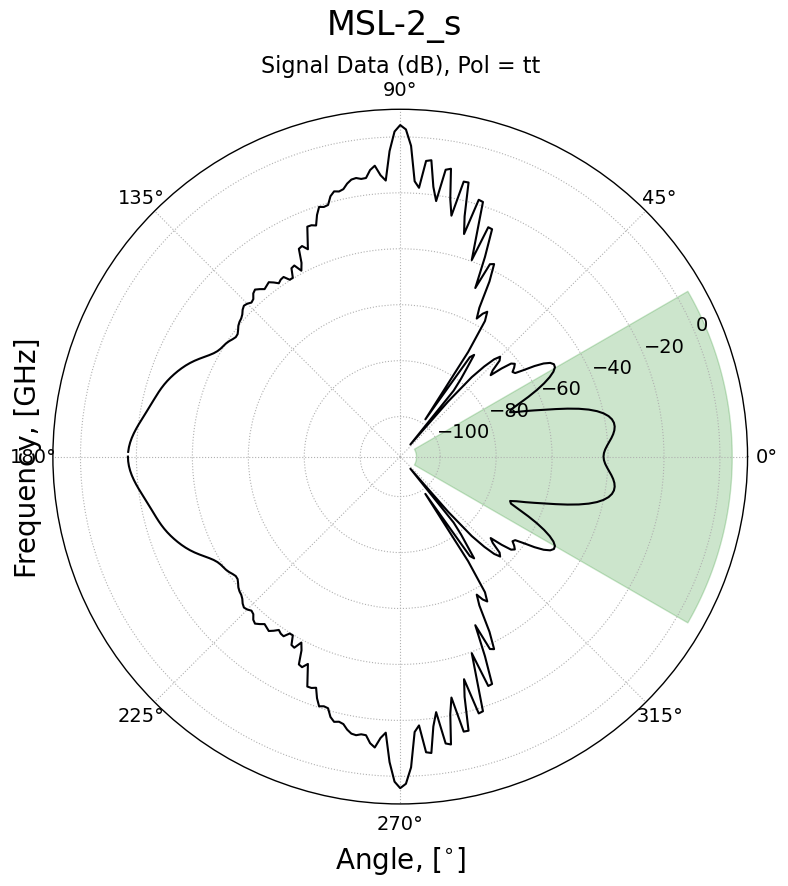
\includegraphics[width=.8\linewidth]{MSL-2_s_dB_tt_5GHz.png}
    \end{subfigure}%
    \begin{subfigure}{.5\textwidth}
      \centering
      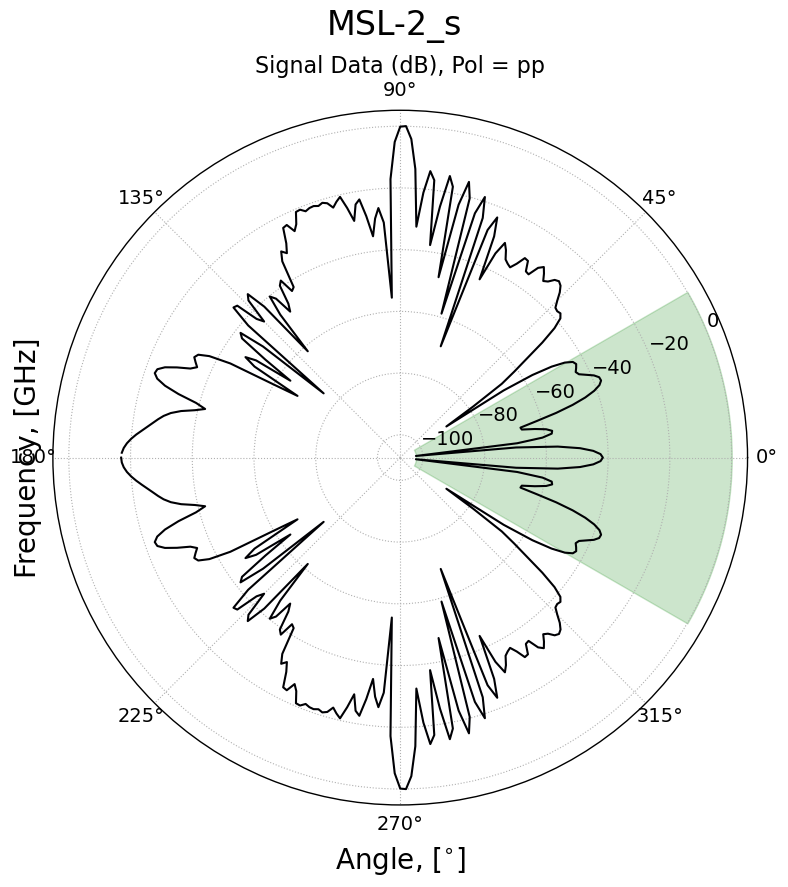
\includegraphics[width=.8\linewidth]{MSL-2_s_dB_pp_5GHz.png}
    \end{subfigure}
    \caption{Missile 2 \textcolor{red}{(Sim)}:  RCS cut at 5 GHz. Vertical (tt) and Horizontal (pp) polarizations }
    \label{fig:ns2}
  \end{figure}

  \begin{figure}[htbp]
    \centering
    \begin{subfigure}{.5\textwidth}
      \centering
      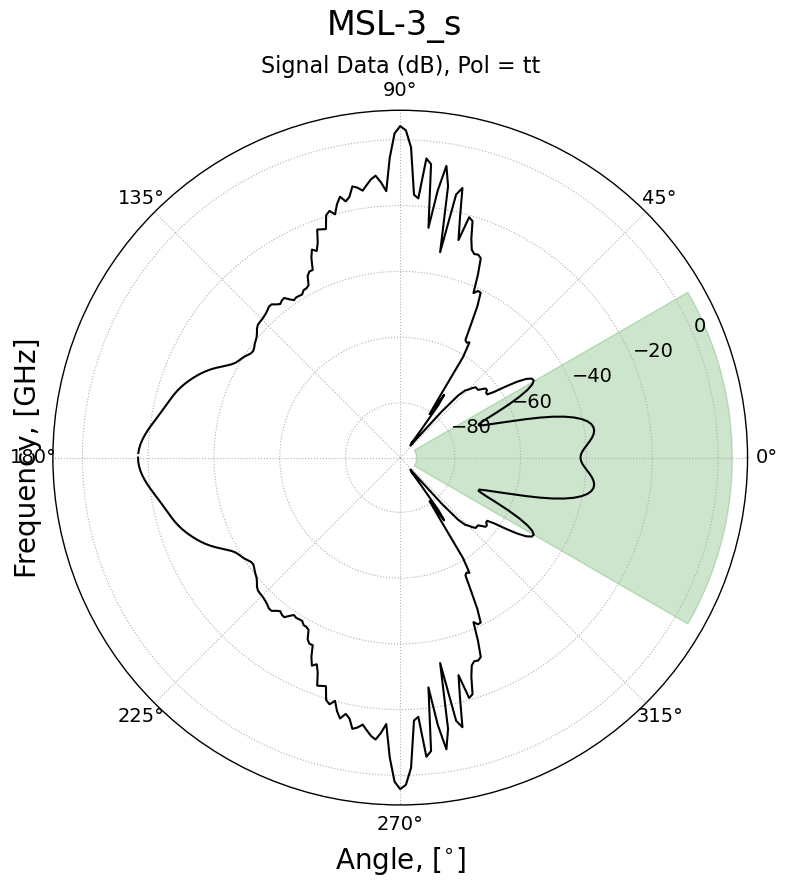
\includegraphics[width=.8\linewidth]{MSL-3_s_dB_tt_5GHz.png}
    \end{subfigure}%
    \begin{subfigure}{.5\textwidth}
      \centering
      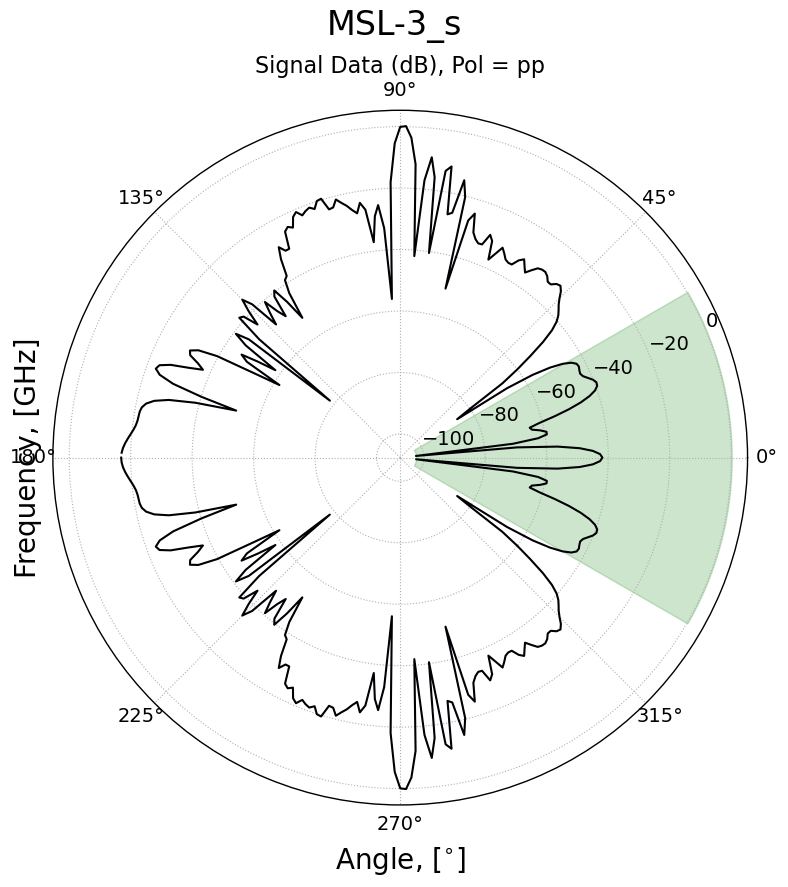
\includegraphics[width=.8\linewidth]{MSL-3_s_dB_pp_5GHz.png}
    \end{subfigure}
    \caption{Missile 3 \textcolor{red}{(Sim)}:  RCS cut at 5 GHz. Vertical (tt) and Horizontal (pp) polarizations }
    \label{fig:ns3}
  \end{figure}

  \begin{figure}[htbp]
    \centering
    \begin{subfigure}{.5\textwidth}
      \centering
      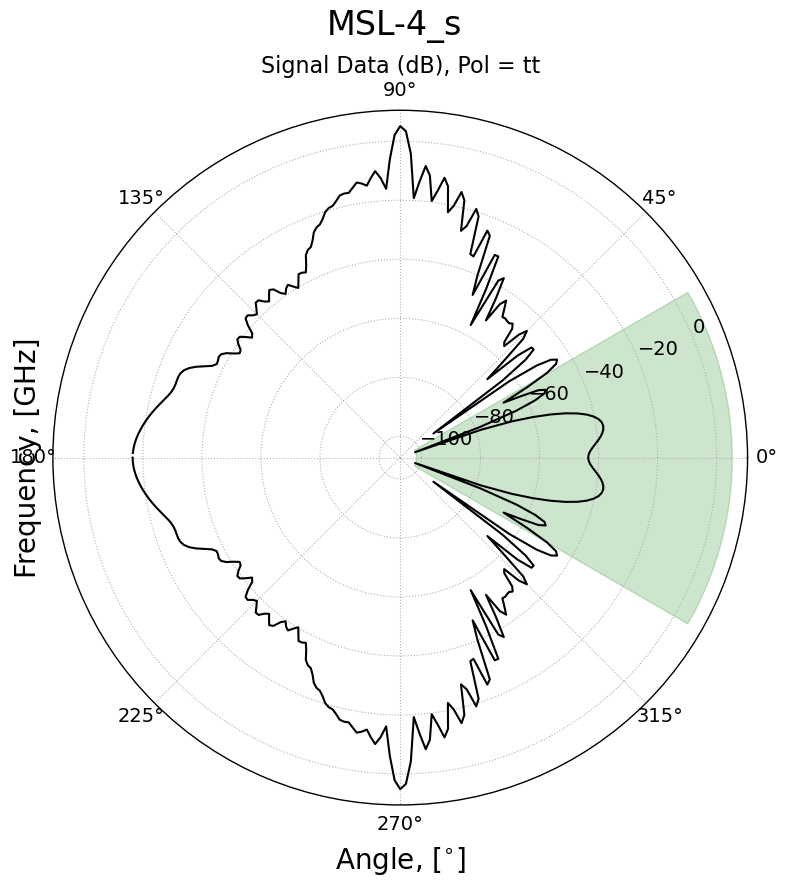
\includegraphics[width=.8\linewidth]{MSL-4_s_dB_tt_5GHz.png}
    \end{subfigure}%
    \begin{subfigure}{.5\textwidth}
      \centering
      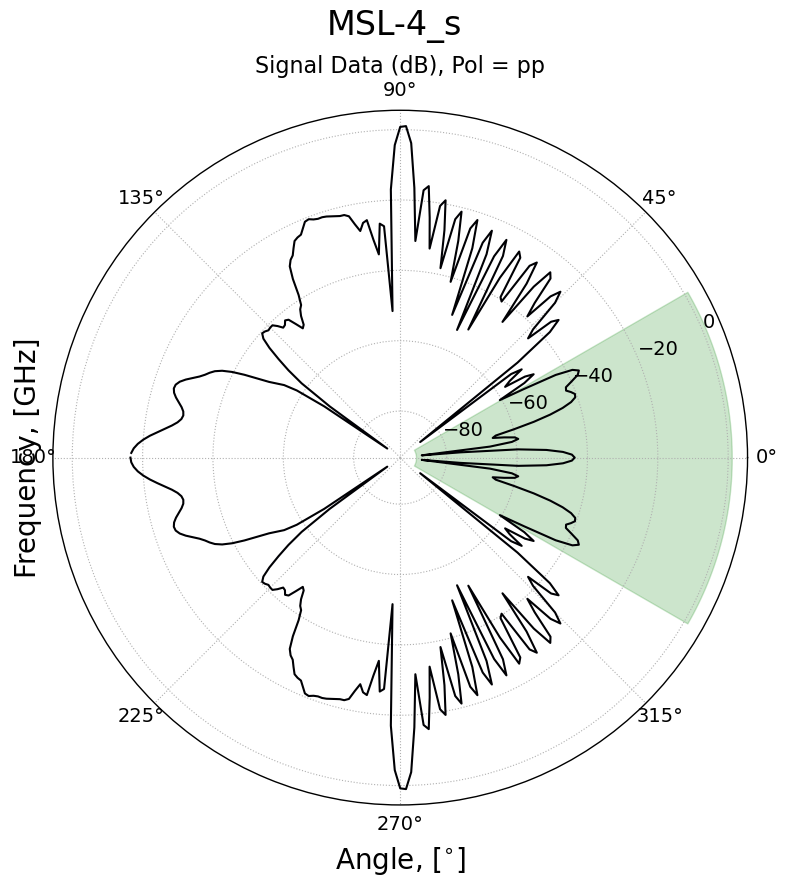
\includegraphics[width=.8\linewidth]{MSL-4_s_dB_pp_5GHz.png}
    \end{subfigure}
    \caption{Missile 4 \textcolor{red}{(Sim)}:  RCS cut at 5 GHz. Vertical (tt) and Horizontal (pp) polarizations }
    \label{fig:ns4}
  \end{figure}

  \begin{figure}[htbp]
    \centering
    \begin{subfigure}{.5\textwidth}
      \centering
      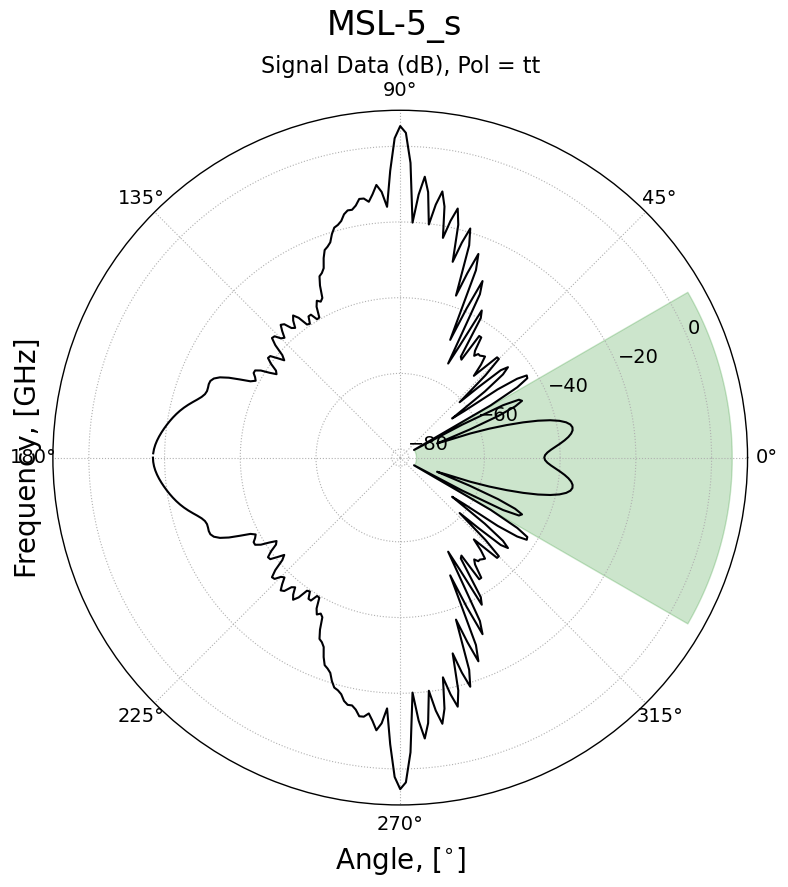
\includegraphics[width=.8\linewidth]{MSL-5_s_dB_tt_5GHz.png}
    \end{subfigure}%
    \begin{subfigure}{.5\textwidth}
      \centering
      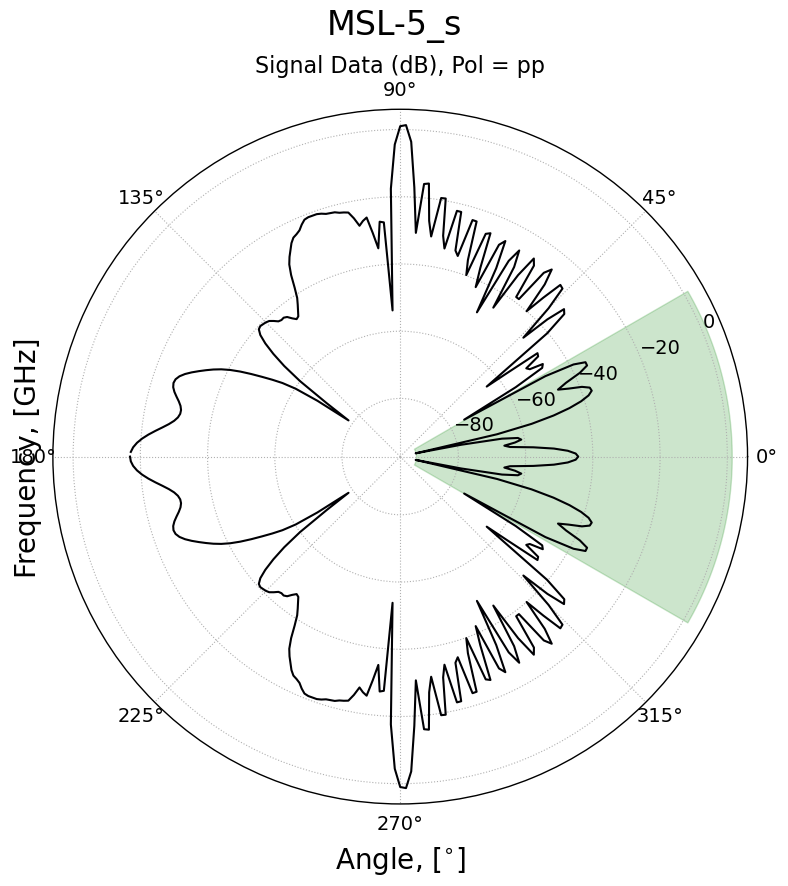
\includegraphics[width=.8\linewidth]{MSL-5_s_dB_pp_5GHz.png}
    \end{subfigure}
    \caption{Missile 5 \textcolor{red}{(Sim)}:  RCS cut at 5 GHz. Vertical (tt) and Horizontal (pp) polarizations }
    \label{fig:ns5}
  \end{figure}

\chapter{Correlation Results}
\label{app:correlation_results}
  \begin{figure}[htbp!]
    \centering
    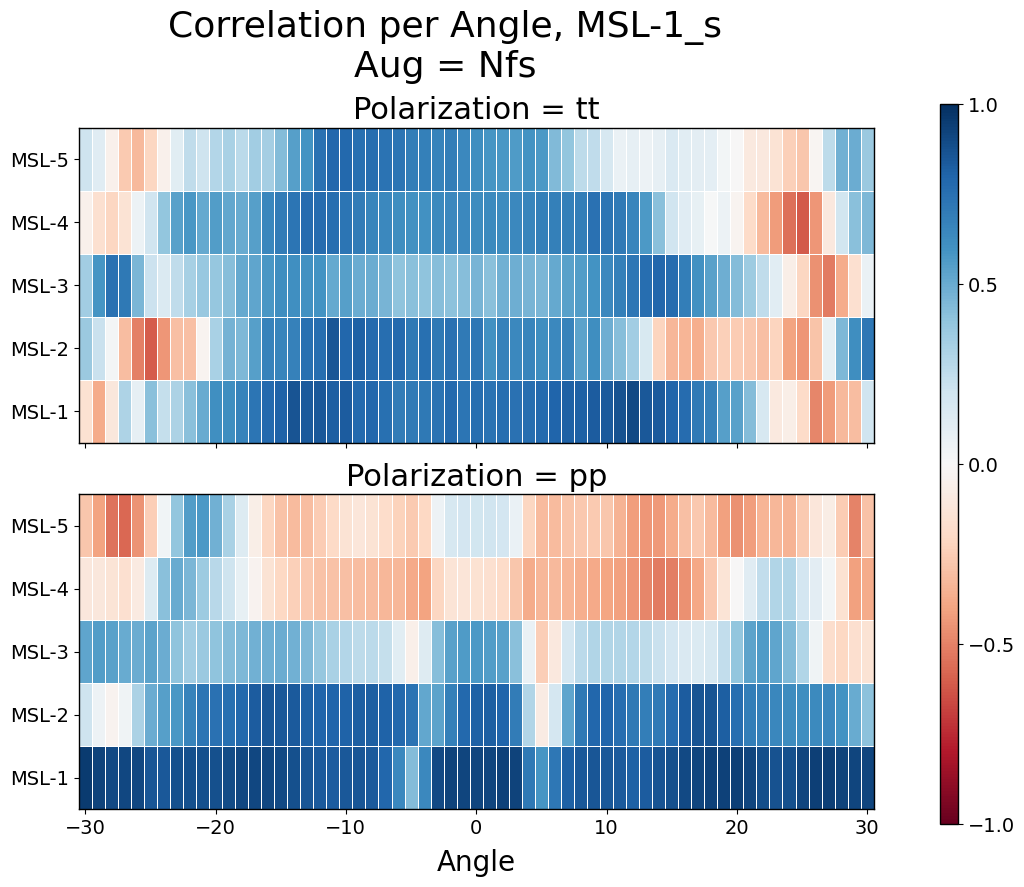
\includegraphics[width=.9\linewidth]{Corr_SNR_MSL-1_s_Nfs.png}
    \caption[Missile 1 Correlations (Sim/Meas)]{Correlation between the simulation of missile 1, and the measured RCS values for each target.}
    \label{fig:corr_msl1}
  \end{figure}

  \begin{figure}[htbp!]
    \centering
    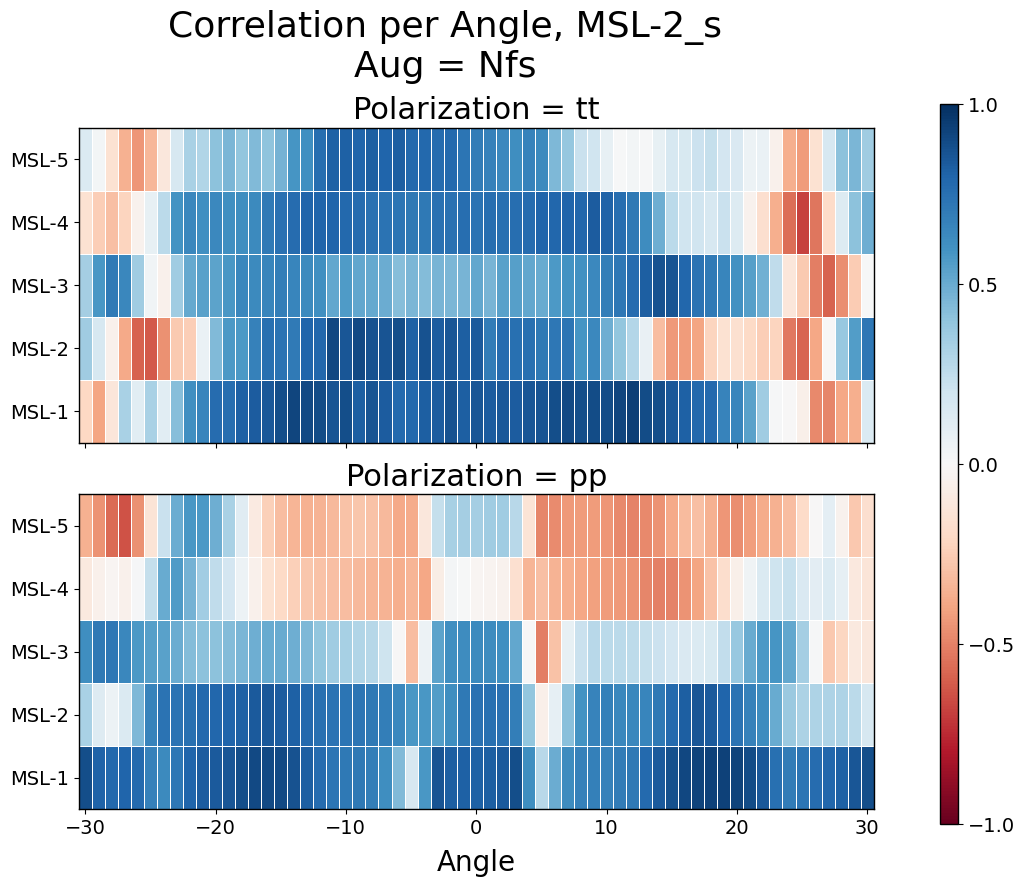
\includegraphics[width=.9\linewidth]{Corr_SNR_MSL-2_s_Nfs.png}
    \caption[Missile 1 Correlations (Sim/Meas)]{Correlation between the simulation of missile 2, and the measured RCS values for each target.}
    \label{fig:corr_msl2}
  \end{figure}

  \begin{figure}[htbp!]
    \centering
    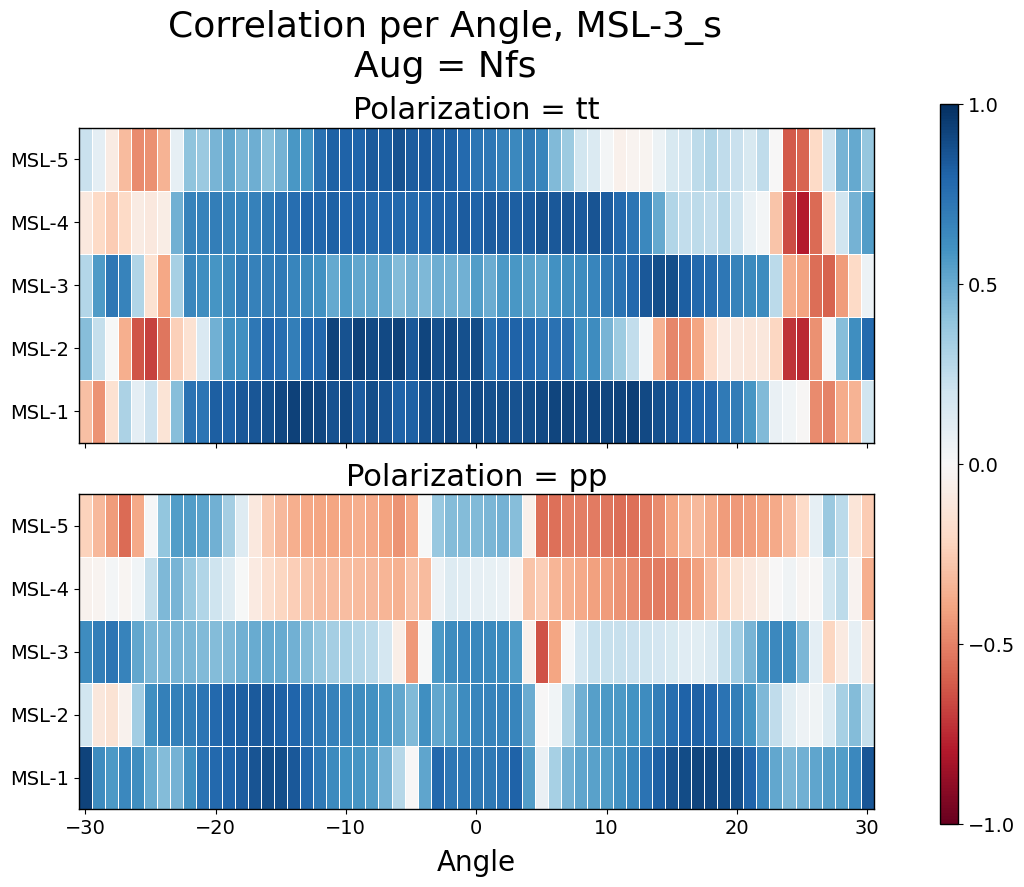
\includegraphics[width=.9\linewidth]{Corr_SNR_MSL-3_s_Nfs.png}
    \caption[Missile 1 Correlations (Sim/Meas)]{Correlation between the simulation of missile 3, and the measured RCS values for each target.}
    \label{fig:corr_msl3}
  \end{figure}

  \begin{figure}[htbp!]
    \centering
    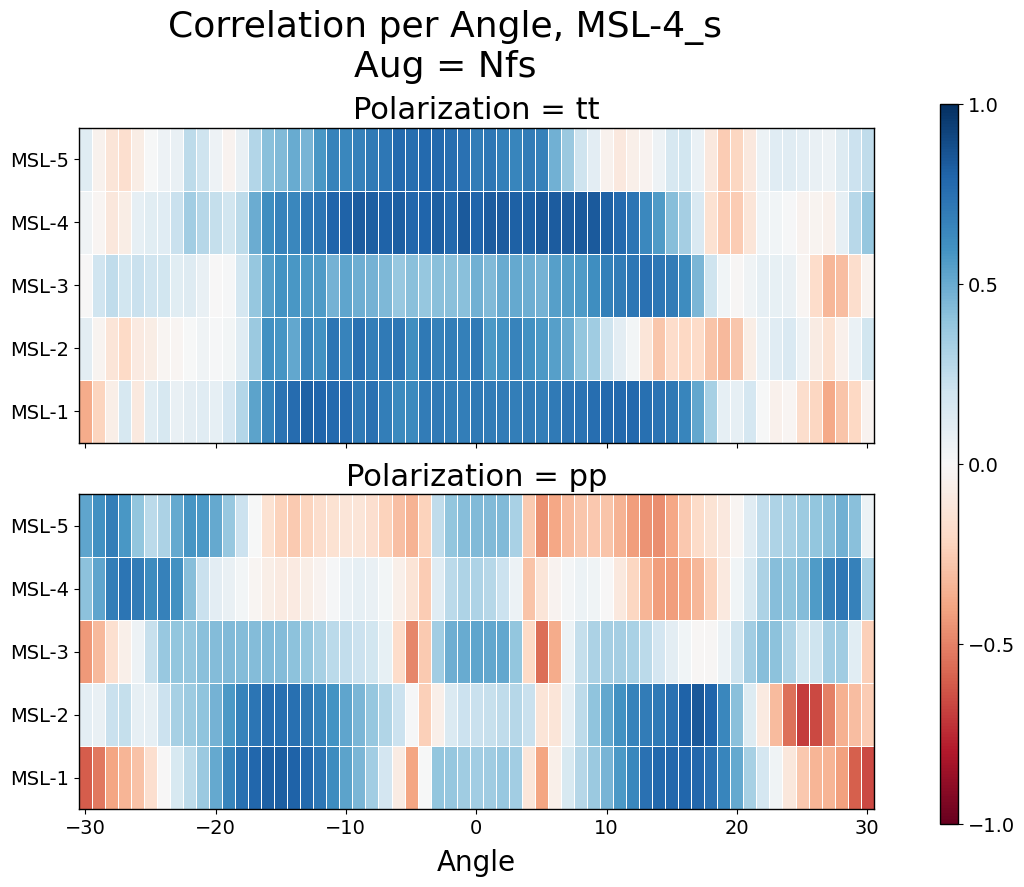
\includegraphics[width=.9\linewidth]{Corr_SNR_MSL-4_s_Nfs.png}
    \caption[Missile 1 Correlations (Sim/Meas)]{Correlation between the simulation of missile 4, and the measured RCS values for each target.}
    \label{fig:corr_msl4}
  \end{figure}

  \begin{figure}[htbp!]
    \centering
    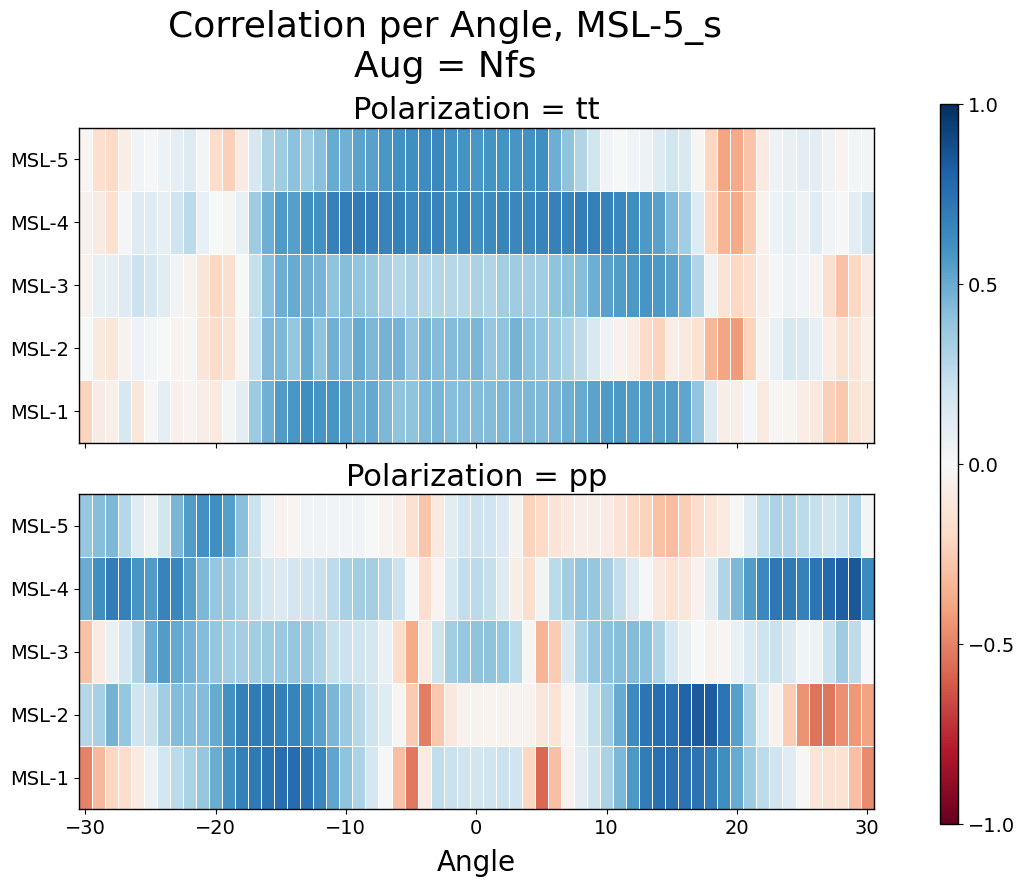
\includegraphics[width=.9\linewidth]{Corr_SNR_MSL-5_s_Nfs.png}
    \caption[Missile 1 Correlations (Sim/Sim)]{Correlation between the simulation of missile 5, and the measured RCS values for each target.}
    \label{fig:corr_msl5}
  \end{figure}

  \begin{figure}[htbp!]
    \centering
    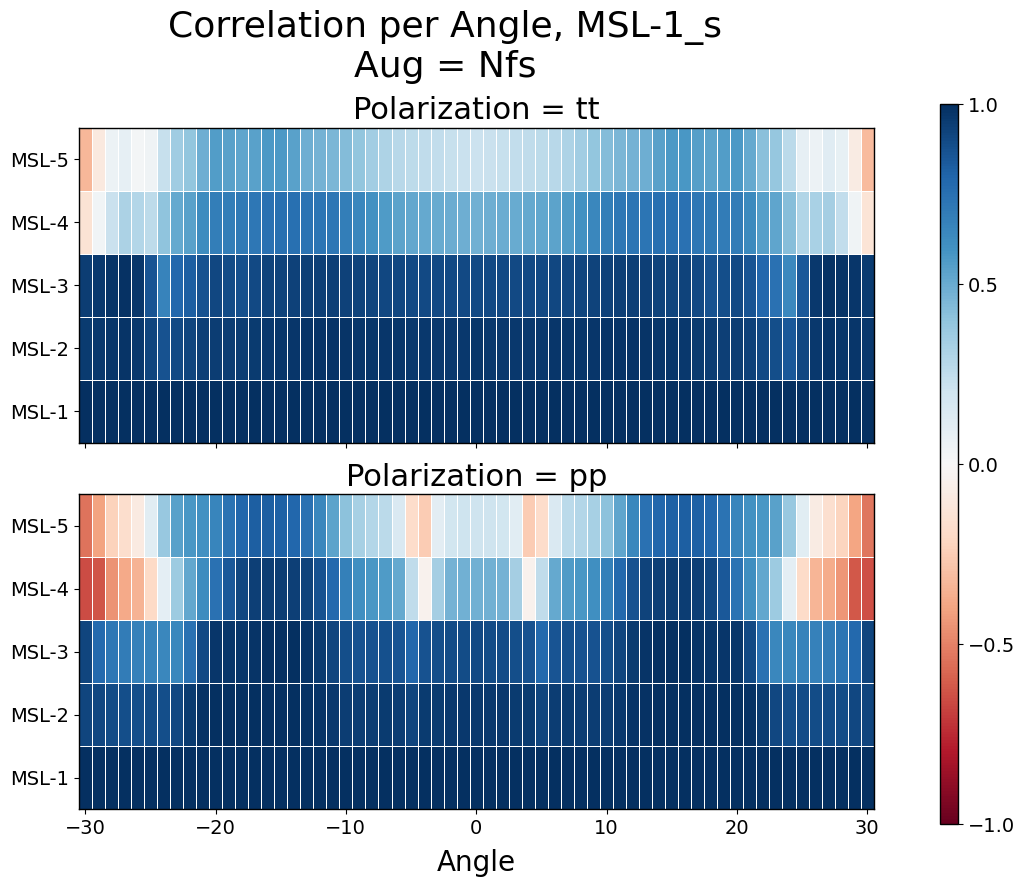
\includegraphics[width=.9\linewidth]{vgg-19_sim_Corr_SNR_MSL-1_s_Nfs.png}
    \caption[Missile 1 Correlations (Sim/Sim)]{Correlation between the simulation of missile 1, and the simulated RCS values for each target.}
    \label{fig:corr_msl1_sim}
  \end{figure}

  \begin{figure}[htbp!]
    \centering
    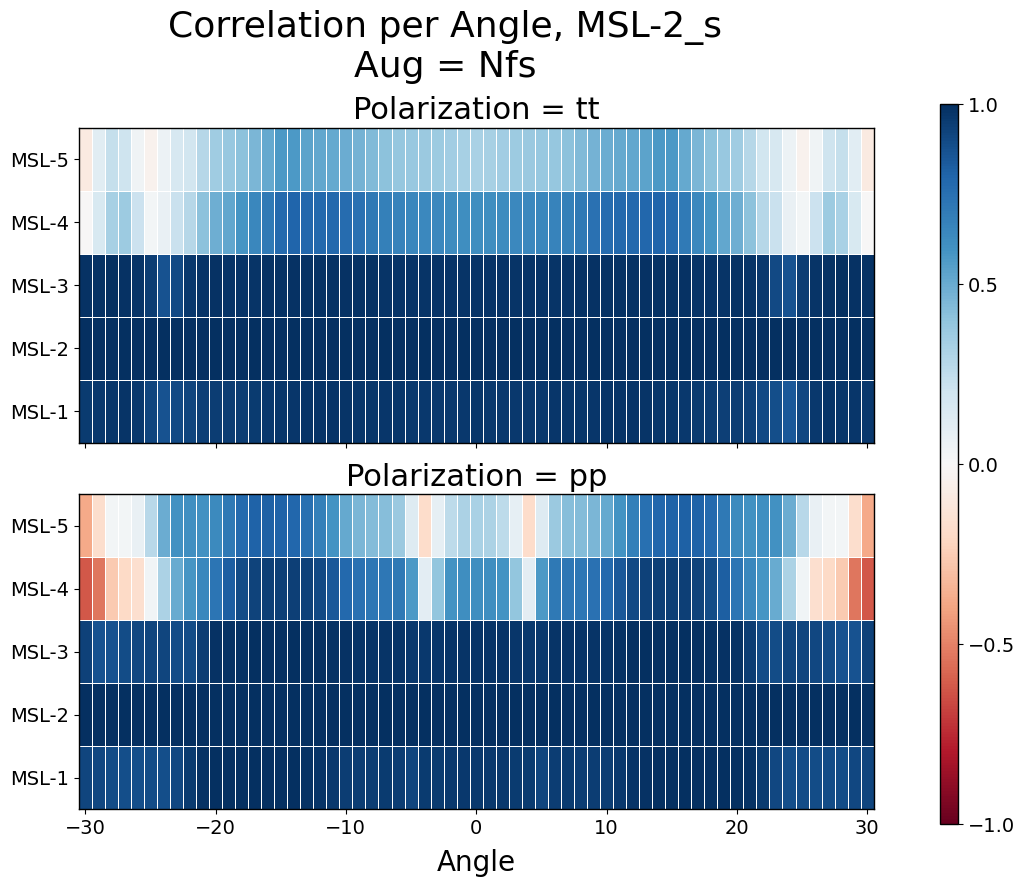
\includegraphics[width=.9\linewidth]{vgg-19_sim_Corr_SNR_MSL-2_s_Nfs.png}
    \caption[Missile 1 Correlations (Sim/Sim)]{Correlation between the simulation of missile 2, and the simulated RCS values for each target.}
    \label{fig:corr_msl2_sim}
  \end{figure}

  \begin{figure}[htbp!]
    \centering
    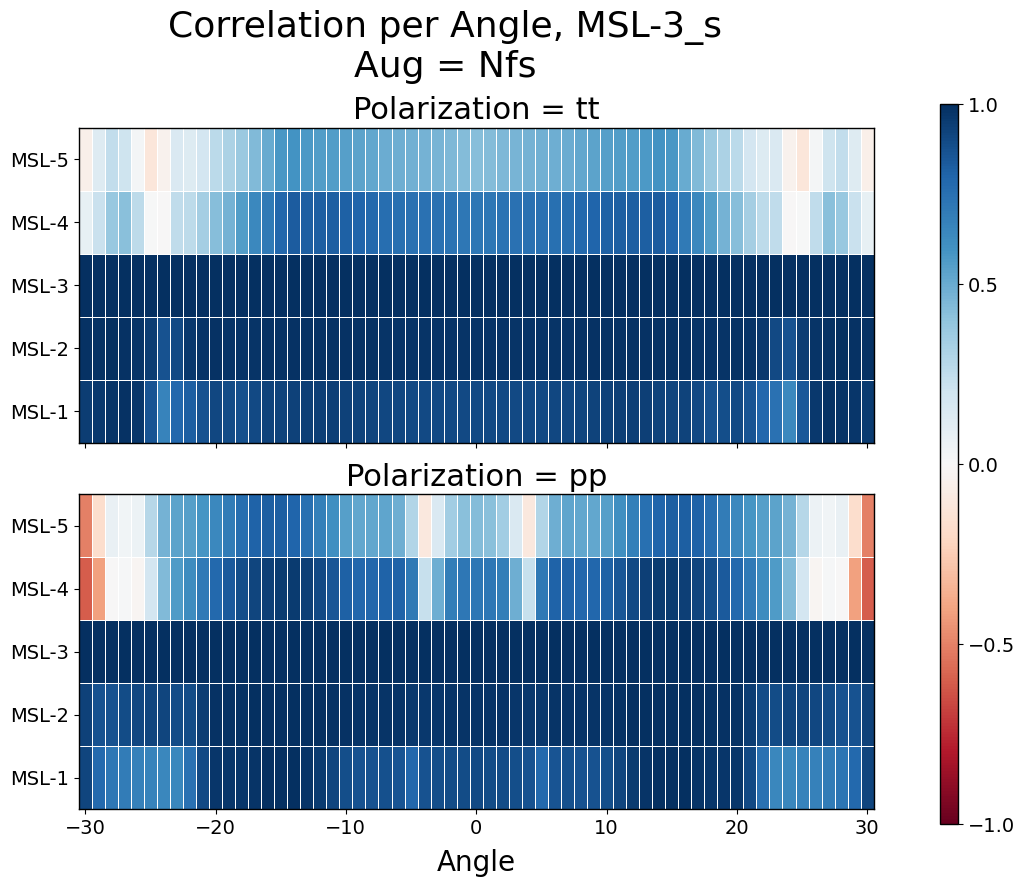
\includegraphics[width=.9\linewidth]{vgg-19_sim_Corr_SNR_MSL-3_s_Nfs.png}
    \caption[Missile 1 Correlations (Sim/Sim)]{Correlation between the simulation of missile 3, and the simulated RCS values for each target.}
    \label{fig:corr_msl3_sim}
  \end{figure}

  \begin{figure}[htbp!]
    \centering
    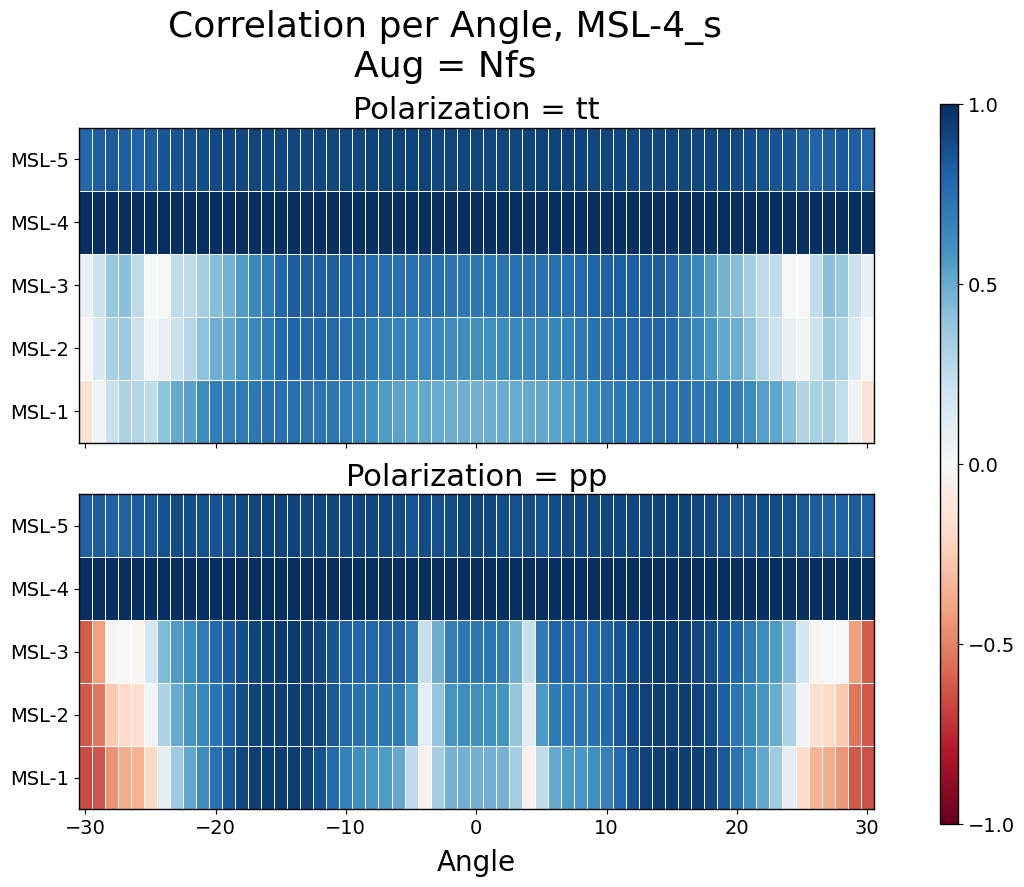
\includegraphics[width=.9\linewidth]{vgg-19_sim_Corr_SNR_MSL-4_s_Nfs.png}
    \caption[Missile 1 Correlations (Sim/Sim)]{Correlation between the simulation of missile 4, and the simulated RCS values for each target.}
    \label{fig:corr_msl4_sim}
  \end{figure}

  \begin{figure}[htbp!]
    \centering
    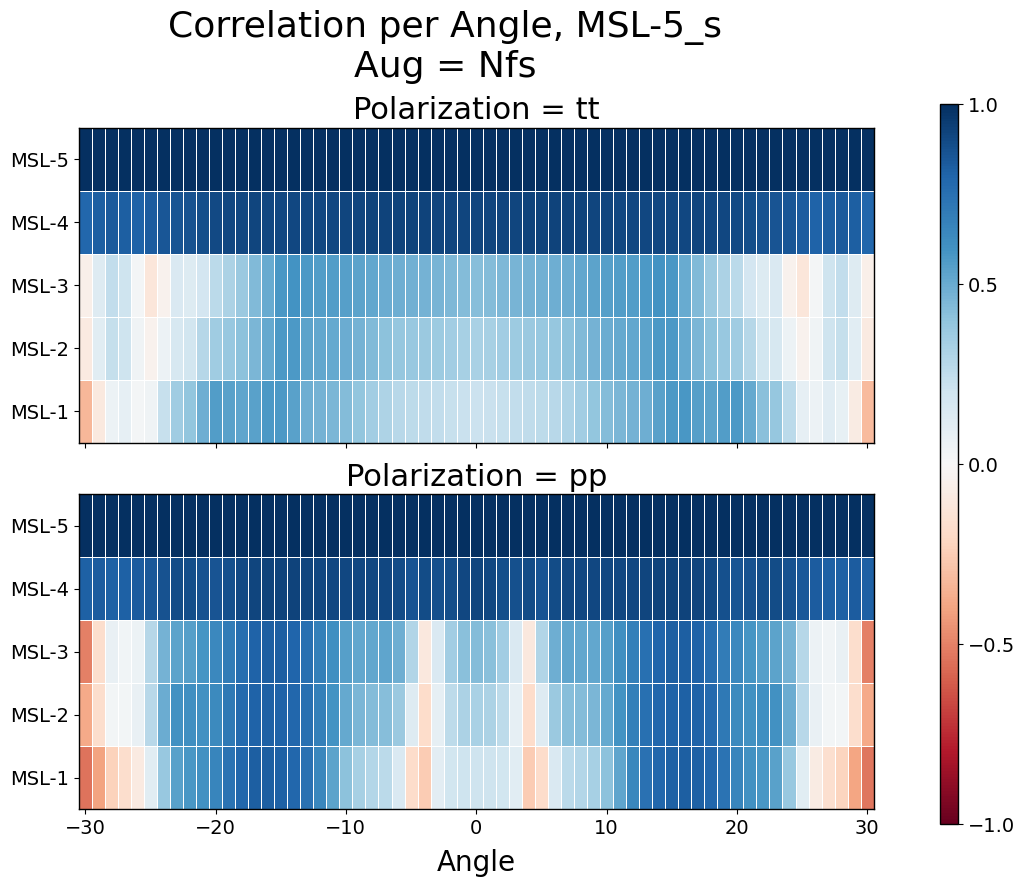
\includegraphics[width=.9\linewidth]{vgg-19_sim_Corr_SNR_MSL-5_s_Nfs.png}
    \caption[Missile 1 Correlations (Sim/Sim)]{Correlation between the simulation of missile 5, and the simulated RCS values for each target.}
    \label{fig:corr_msl5_sim}
  \end{figure}

\chapter{VGG-19 Results}
\label{app:vgg-19_results}

  \begin{figure}[htbp!]
    \centering
    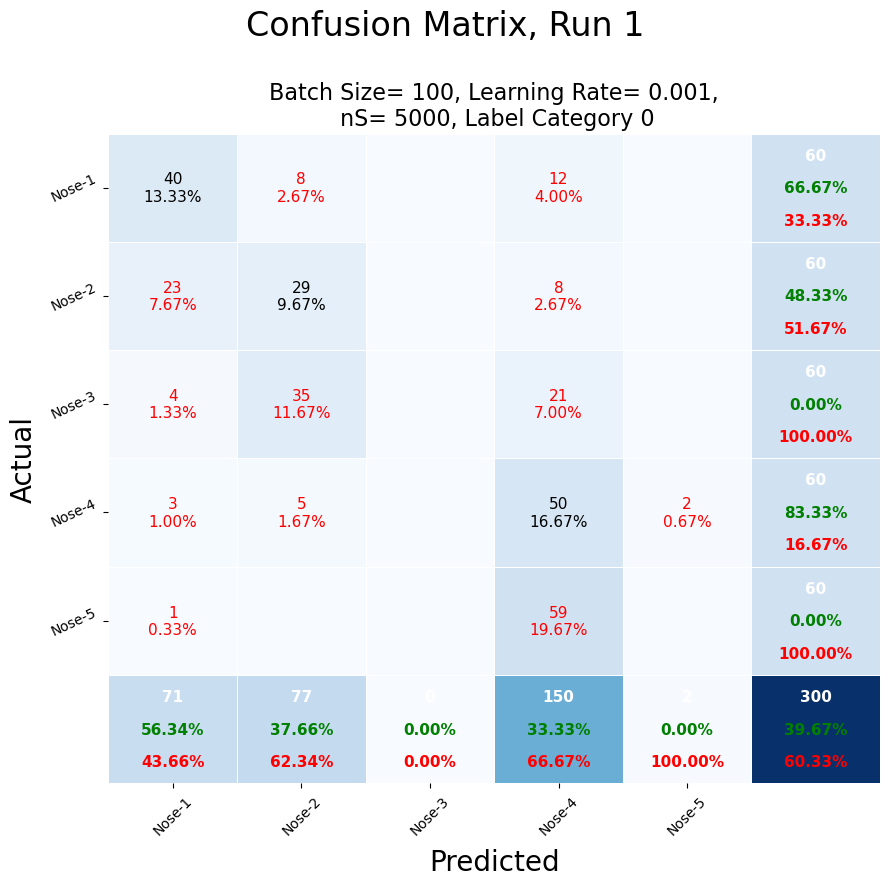
\includegraphics[width=.9\linewidth]{19_1_CM.png}
    \caption[VGG-19, -10 dBm Confusion Matrix]{Confusion matrix for the -10 dBm model in the VGG-19 siamese network.}
    \label{fig:vgg-19_cm1}
  \end{figure}

  \begin{figure}[htbp!]
    \centering
    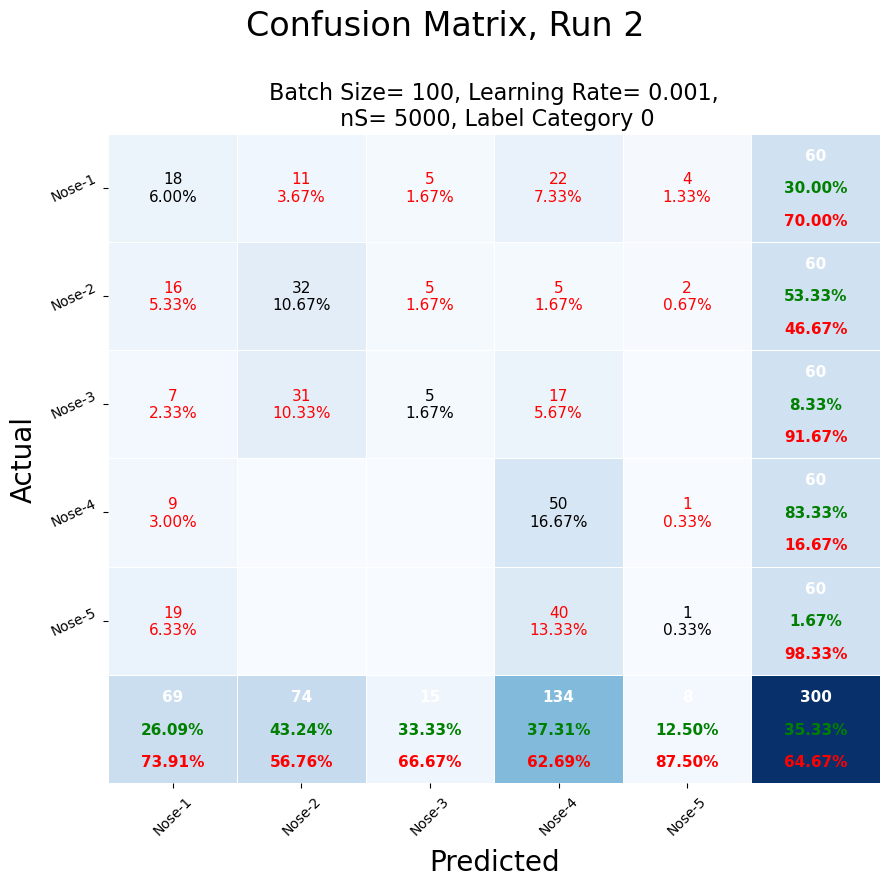
\includegraphics[width=.9\linewidth]{19_2_CM.png}
    \caption[VGG-19, -5 dBm Confusion Matrix]{Confusion matrix for the -5 dBm model in the VGG-19 siamese network.}
    \label{fig:vgg-19_cm2}
  \end{figure}

  \begin{figure}[htbp!]
    \centering
    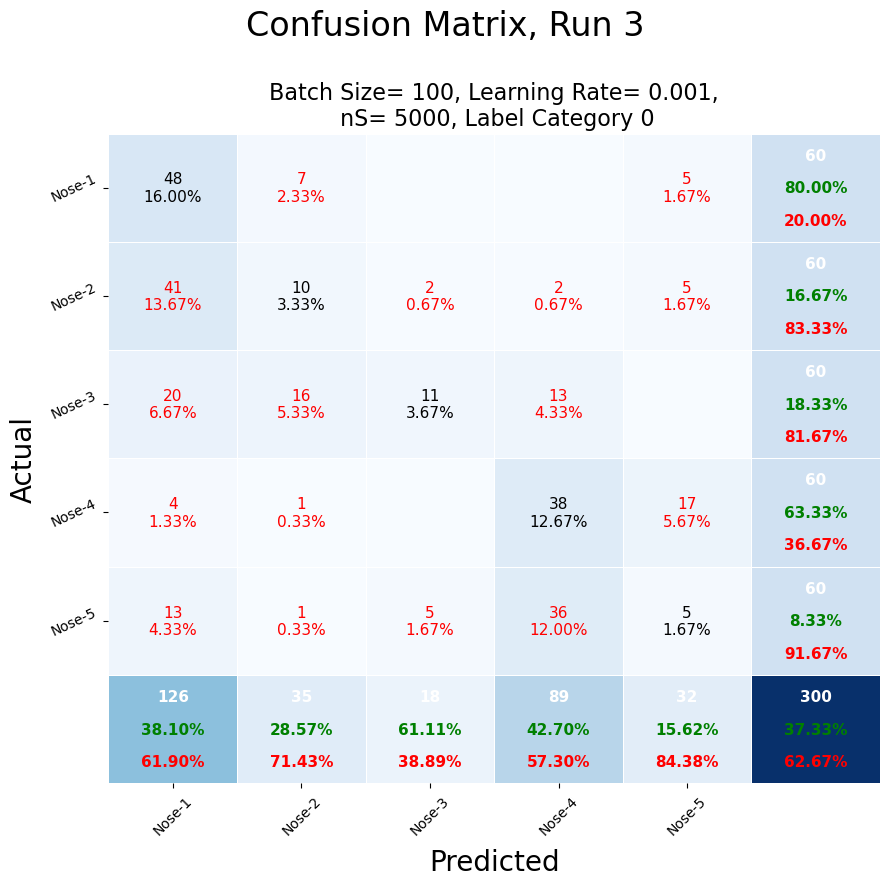
\includegraphics[width=.9\linewidth]{19_3_CM.png}
    \caption[VGG-19, 0 dBm Confusion Matrix]{Confusion matrix for the 0 dBm model in the VGG-19 siamese network.}
    \label{fig:vgg-19_cm3}
  \end{figure}

  \begin{figure}[htbp!]
    \centering
    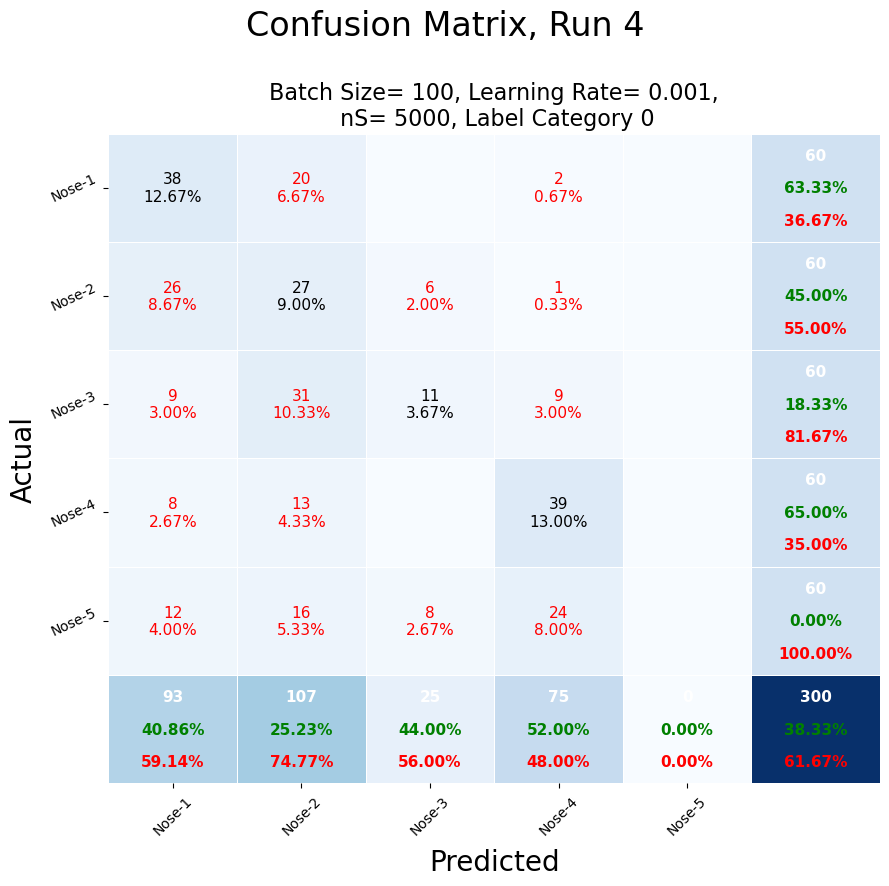
\includegraphics[width=.9\linewidth]{19_4_CM.png}
    \caption[VGG-19, 5 dBm Confusion Matrix]{Confusion matrix for the 5 dBm model in the VGG-19 siamese network.}
    \label{fig:vgg-19_cm4}
  \end{figure}

  \begin{figure}[htbp!]
    \centering
    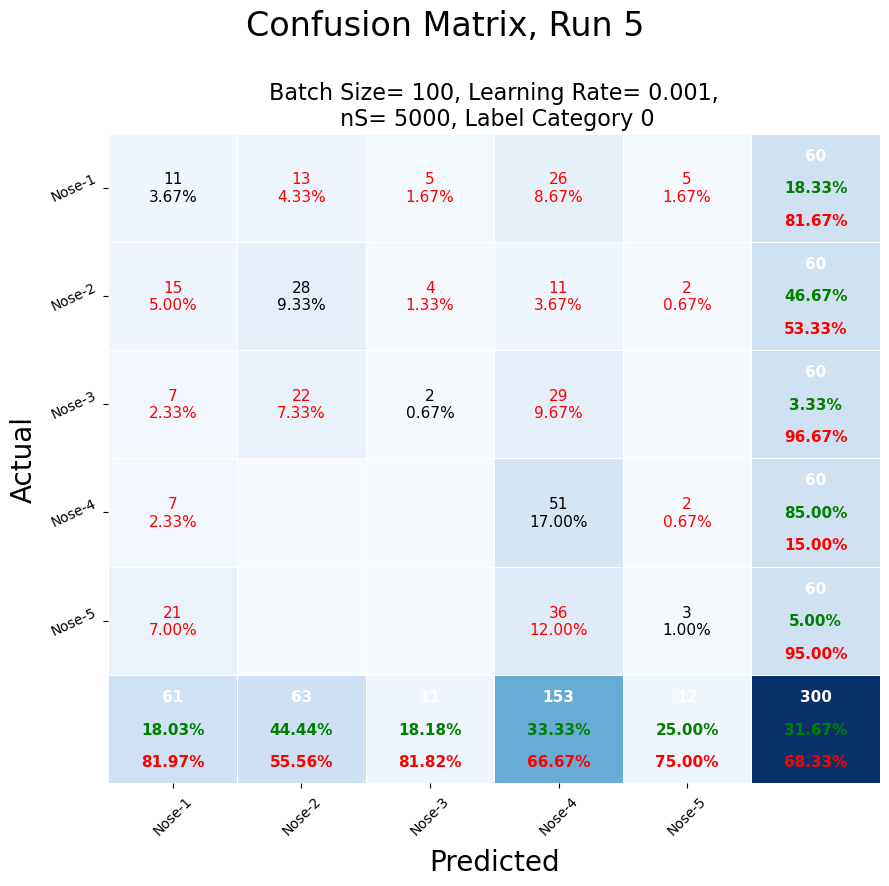
\includegraphics[width=.9\linewidth]{19_5_CM.png}
    \caption[VGG-19, 10 dBm Confusion Matrix]{Confusion matrix for the 10 dBm model in the VGG-19 siamese network.}
    \label{fig:vgg-19_cm5}
  \end{figure}

  \begin{figure}[htbp]
    \centering
    \begin{subfigure}{.5\textwidth}
      \centering
      \includegraphics[width=.9\linewidth]{vgg-19_meas_Angle_ACC_-10.png}
    \end{subfigure}%
    \begin{subfigure}{.5\textwidth}
      \centering
      \includegraphics[width=.9\linewidth]{vgg-19_meas_Pred_Angle_-10.png}
    \end{subfigure}
    \caption{Angle accuracy and Classification for the VGG-19 siamese network, SNR=-10 dB}
    \label{fig:vgg-19_snr1}
  \end{figure}

  \begin{figure}[htbp]
    \centering
    \begin{subfigure}{.5\textwidth}
      \centering
      \includegraphics[width=.9\linewidth]{vgg-19_meas_Angle_ACC_-8.png}
    \end{subfigure}%
    \begin{subfigure}{.5\textwidth}
      \centering
      \includegraphics[width=.9\linewidth]{vgg-19_meas_Pred_Angle_-8.png}
    \end{subfigure}
    \caption{Angle accuracy and Classification for the VGG-19 siamese network, SNR=-8 dB}
    \label{fig:vgg-19_snr2}
  \end{figure}

  \begin{figure}[htbp]
    \centering
    \begin{subfigure}{.5\textwidth}
      \centering
      \includegraphics[width=.9\linewidth]{vgg-19_meas_Angle_ACC_-6.png}
    \end{subfigure}%
    \begin{subfigure}{.5\textwidth}
      \centering
      \includegraphics[width=.9\linewidth]{vgg-19_meas_Pred_Angle_-6.png}
    \end{subfigure}
    \caption{Angle accuracy and Classification for the VGG-19 siamese network, SNR=-6 dB}
    \label{fig:vgg-19_snr3}
  \end{figure}

  \begin{figure}[htbp]
    \centering
    \begin{subfigure}{.5\textwidth}
      \centering
      \includegraphics[width=.9\linewidth]{vgg-19_meas_Angle_ACC_-4.png}
    \end{subfigure}%
    \begin{subfigure}{.5\textwidth}
      \centering
      \includegraphics[width=.9\linewidth]{vgg-19_meas_Pred_Angle_-4.png}
    \end{subfigure}
    \caption{Angle accuracy and Classification for the VGG-19 siamese network, SNR=-4 dB}
    \label{fig:vgg-19_snr4}
  \end{figure}

  \begin{figure}[htbp]
    \centering
    \begin{subfigure}{.5\textwidth}
      \centering
      \includegraphics[width=.9\linewidth]{vgg-19_meas_Angle_ACC_-2.png}
    \end{subfigure}%
    \begin{subfigure}{.5\textwidth}
      \centering
      \includegraphics[width=.9\linewidth]{vgg-19_meas_Pred_Angle_-2.png}
    \end{subfigure}
    \caption{Angle accuracy and Classification for the VGG-19 siamese network, SNR=-2 dB}
    \label{fig:vgg-19_snr5}
  \end{figure}

  \begin{figure}[htbp]
    \centering
    \begin{subfigure}{.5\textwidth}
      \centering
      \includegraphics[width=.9\linewidth]{vgg-19_meas_Angle_ACC_0.png}
    \end{subfigure}%
    \begin{subfigure}{.5\textwidth}
      \centering
      \includegraphics[width=.9\linewidth]{vgg-19_meas_Pred_Angle_0.png}
    \end{subfigure}
    \caption{Angle accuracy and Classification for the VGG-19 siamese network, SNR=0 dB}
    \label{fig:vgg-19_snr6}
  \end{figure}

  \begin{figure}[htbp]
    \centering
    \begin{subfigure}{.5\textwidth}
      \centering
      \includegraphics[width=.9\linewidth]{vgg-19_meas_Angle_ACC_3.png}
    \end{subfigure}%
    \begin{subfigure}{.5\textwidth}
      \centering
      \includegraphics[width=.9\linewidth]{vgg-19_meas_Pred_Angle_3.png}
    \end{subfigure}
    \caption{Angle accuracy and Classification for the VGG-19 siamese network, SNR=3 dB}
    \label{fig:vgg-19_snr7}
  \end{figure}

  \begin{figure}[htbp]
    \centering
    \begin{subfigure}{.5\textwidth}
      \centering
      \includegraphics[width=.9\linewidth]{vgg-19_meas_Angle_ACC_5.png}
    \end{subfigure}%
    \begin{subfigure}{.5\textwidth}
      \centering
      \includegraphics[width=.9\linewidth]{vgg-19_meas_Pred_Angle_5.png}
    \end{subfigure}
    \caption{Angle accuracy and Classification for the VGG-19 siamese network, SNR=5 dB}
    \label{fig:vgg-19_snr8}
  \end{figure}

  \begin{figure}[htbp]
    \centering
    \begin{subfigure}{.5\textwidth}
      \centering
      \includegraphics[width=.9\linewidth]{vgg-19_meas_Angle_ACC_7.png}
    \end{subfigure}%
    \begin{subfigure}{.5\textwidth}
      \centering
      \includegraphics[width=.9\linewidth]{vgg-19_meas_Pred_Angle_7.png}
    \end{subfigure}
    \caption{Angle accuracy and Classification for the VGG-19 siamese network, SNR=7 dB}
    \label{fig:vgg-19_snr9}
  \end{figure}

  \begin{figure}[htbp]
    \centering
    \begin{subfigure}{.5\textwidth}
      \centering
      \includegraphics[width=.9\linewidth]{vgg-19_meas_Angle_ACC_9.png}
    \end{subfigure}%
    \begin{subfigure}{.5\textwidth}
      \centering
      \includegraphics[width=.9\linewidth]{vgg-19_meas_Pred_Angle_9.png}
    \end{subfigure}
    \caption{Angle accuracy and Classification for the VGG-19 siamese network, SNR=9 dB}
    \label{fig:vgg-19_snr10}
  \end{figure}

  \begin{figure}[htbp]
    \centering
    \begin{subfigure}{.5\textwidth}
      \centering
      \includegraphics[width=.9\linewidth]{vgg-19_meas_Angle_ACC_11.png}
    \end{subfigure}%
    \begin{subfigure}{.5\textwidth}
      \centering
      \includegraphics[width=.9\linewidth]{vgg-19_meas_Pred_Angle_11.png}
    \end{subfigure}
    \caption{Angle accuracy and Classification for the VGG-19 siamese network, SNR=11 dB}
    \label{fig:vgg-19_snr11}
  \end{figure}

  \begin{figure}[htbp]
    \centering
    \begin{subfigure}{.5\textwidth}
      \centering
      \includegraphics[width=.9\linewidth]{vgg-19_meas_Angle_ACC_13.png}
    \end{subfigure}%
    \begin{subfigure}{.5\textwidth}
      \centering
      \includegraphics[width=.9\linewidth]{vgg-19_meas_Pred_Angle_13.png}
    \end{subfigure}
    \caption{Angle accuracy and Classification for the VGG-19 siamese network, SNR=13 dB}
    \label{fig:vgg-19_snr12}
  \end{figure}

  \begin{figure}[htbp]
    \centering
    \begin{subfigure}{.5\textwidth}
      \centering
      \includegraphics[width=.9\linewidth]{vgg-19_meas_Angle_ACC_15.png}
    \end{subfigure}%
    \begin{subfigure}{.5\textwidth}
      \centering
      \includegraphics[width=.9\linewidth]{vgg-19_meas_Pred_Angle_15.png}
    \end{subfigure}
    \caption{Angle accuracy and Classification for the VGG-19 siamese network, SNR=15 dB}
    \label{fig:vgg-19_snr13}
  \end{figure}

  \begin{figure}[htbp]
    \centering
    \begin{subfigure}{.5\textwidth}
      \centering
      \includegraphics[width=.9\linewidth]{vgg-19_meas_Angle_ACC_18.png}
    \end{subfigure}%
    \begin{subfigure}{.5\textwidth}
      \centering
      \includegraphics[width=.9\linewidth]{vgg-19_meas_Pred_Angle_18.png}
    \end{subfigure}
    \caption{Angle accuracy and Classification for the VGG-19 siamese network, SNR=18 dB}
    \label{fig:vgg-19_snr14}
  \end{figure}

  \begin{figure}[htbp]
    \centering
    \begin{subfigure}{.5\textwidth}
      \centering
      \includegraphics[width=.9\linewidth]{vgg-19_meas_Angle_ACC_20.png}
    \end{subfigure}%
    \begin{subfigure}{.5\textwidth}
      \centering
      \includegraphics[width=.9\linewidth]{vgg-19_meas_Pred_Angle_20.png}
    \end{subfigure}
    \caption{Angle accuracy and Classification for the VGG-19 siamese network, SNR=20 dB}
    \label{fig:vgg-19_snr15}
  \end{figure}

\chapter{VGG-16 Results}
\label{app:vgg-16_results}

  \begin{table}
    \centering
    \begin{tabular}{|r|r|r|r|}
      \hline
      Run number &	Sample Size	& Training Noise [dBm] & Momentum \\
      \hline
      1	& 2000 	& 0.5	& -5 \\
      \hline
      2	& 2000 	& 0.7	& -10 \\
      \hline
      3	& 1000 	& 0.7	& 10 \\
      \hline
      4	& 1000 	& 0.5	& -5 \\
      \hline
      5	& 2000 	& 0.5	& -10 \\
      \hline
      6	& 1000 	& 0.7	& -5 \\
      \hline
      7	& 2000 	& 0.7	& 0 \\
      \hline
      8	& 2000 	& 0.5	& 0 \\
      \hline
      9	& 1000 	& 0.5	& 0 \\
      \hline
      10	& 2000 	& 0.7	& -5 \\
      \hline
      11	& 2000 	& 0.5	& 10 \\
      \hline
      12	& 1000 	& 0.7	& -10 \\
      \hline
      13	& 2000 	& 0.5	& 5 \\
      \hline
      14	& 1000 	& 0.5	& 10 \\
      \hline
      15	& 1000 	& 0.5	& -10 \\
      \hline
      16	& 1000 	& 0.5	& 5 \\
      \hline
      17	& 2000 	& 0.7	& 10 \\
      \hline
      18	& 1000 	& 0.7	& 0 \\
      \hline
      19	& 1000 	& 0.7	& 5 \\
      \hline
      20	& 2000 	& 0.7	& 5 \\
      \hline
    \end{tabular}
    \caption{VGG-16 test card listing teh evaluted configurations of the network.}
    \label{tab:vgg-16_test_card}
  \end{table}
